%&preformat-present

\newif\ifpresentation % Условие, проверяющее, что документ --- презентация
\presentationtrue
\documentclass[10pt, xcolor={dvipsnames, table, hyperref}]{beamer}

%%% Добавление поясняющих записей (notes) к презентации %%%
\makeatletter
\@ifundefined{c@presnotes}{
    \newcounter{presnotes}
    \setcounter{presnotes}{0}       % 0 --- выкл;
                                    % 1 --- вкл, записи на отдельном слайде;
                                    % 2 --- вкл, записи на основном слайде;
}{}
\makeatother

%%% Положение поясняющих записей (notes) при значении presnotes=2 %%%
\newcommand{\presposition}{left}  % возможные значения: left, right, top, bottom

%%% Добавление логотипа из файла images/logo на первом слайде %%%
\makeatletter
\@ifundefined{c@logotitle}{
    \newcounter{logotitle}
    \setcounter{logotitle}{1}       % 0 --- выкл;
                                    % 1 --- вкл
}{}
\makeatother

%%% Добавление логотипа из файла images/logo на слайдах (кроме первого и последнего) %%%
\makeatletter
\@ifundefined{c@logoother}{
    \newcounter{logoother}
    \setcounter{logoother}{0}       % 0 --- выкл;
                                    % 1 --- вкл
}{}
\makeatother
               % Общие настройки шаблона
%%% Проверка используемого TeX-движка %%%
\usepackage{ifxetex}

%%% Поля и разметка страницы %%%
\usepackage{lscape}                                % Для включения альбомных страниц
\usepackage{geometry}                              % Для последующего задания полей
\usepackage{float}

%%% Математические пакеты %%%
\usepackage{amsthm,amsfonts,amsmath,amssymb,amscd} % Математические дополнения от AMS

%%% Кодировки и шрифты %%%
\ifxetex
  \usepackage{polyglossia}                         % Поддержка многоязычности
  \usepackage{fontspec}                            % TrueType-шрифты
\else
  \usepackage{cmap}                                % Улучшенный поиск русских слов в полученном pdf-файле
  \usepackage[T2A]{fontenc}                        % Поддержка русских букв
  \usepackage[utf8]{inputenc}                      % Кодировка utf8
  \usepackage[english, russian]{babel}             % Языки: русский, английский
  \usepackage{pscyr}                               % Красивые русские шрифты
\fi

%%% Оформление абзацев %%%
\usepackage{indentfirst}                           % Красная строка

%%% Цвета %%%
\usepackage[usenames]{color}
\usepackage{color}
\usepackage{colortbl}

%%% Таблицы %%%
\usepackage{longtable}                             % Длинные таблицы
\usepackage{multirow,makecell,array}               % Улучшенное форматирование таблиц

%%% Общее форматирование
\usepackage[singlelinecheck=off,center]{caption}   % Многострочные подписи
\usepackage{soul}                                  % Поддержка переносоустойчивых подчёркиваний и зачёркиваний
\usepackage{icomma}                                % Запятая в десятичных дробях

%%% Библиография %%%
\usepackage{cite}

%%% Гиперссылки %%%
\usepackage[plainpages=false,pdfpagelabels=false]{hyperref}

%%% Изображения %%%
\usepackage{graphicx}                              % Подключаем пакет работы с графикой

%%% Опционально %%%
% Следующий пакет может быть полезен, если надо ужать текст, чтобы сам текст не править, но чтобы места он занимал поменьше
%\usepackage{savetrees}

% Этот пакет может быть полезен для печати текста брошюрой
%\usepackage[print]{booklet}            % Пакеты общие для диссертации и автореферата
%%% Основные сведения %%%
\newcommand{\thesisAuthor}             % Диссертация, ФИО автора
{Григорьев Семён Вячеславович}
\newcommand{\thesisTitle}              % Диссертация, название
{Cинтаксический анализ динамически формируемых строковых выражений}
\newcommand{\thesisSpecialtyNumber}    % Диссертация, специальность, номер
{05.13.11}
\newcommand{\thesisSpecialtyTitle}     % Диссертация, специальность, название
{Математическое и программное обеспечение вычислительных машин, комплексов и компьютерных сетей}
\newcommand{\thesisDegree}             % Диссертация, научная степень
{кандидата физико-математических наук}
\newcommand{\thesisCity}               % Диссертация, город защиты
{Санкт-Петербург}
\newcommand{\thesisYear}               % Диссертация, год защиты
{2015}
\newcommand{\thesisOrganization}       % Диссертация, организация
{кафедре системного программирования математико-механического факультета Санкт-Петербургского государственного университета}

\newcommand{\supervisorFio}            % Научный руководитель, ФИО
{Кознов Дмитрий Владимирович}
\newcommand{\supervisorRegalia}        % Научный руководитель, регалии
{кандидат физико-математических наук, доцент}

\newcommand{\opponentOneFio}           % Оппонент 1, ФИО
{Лисс Александр Рудольфович}
\newcommand{\opponentOneRegalia}       % Оппонент 1, регалии
{доктор технических наук, профессор, начальник исследовательского отделения}
\newcommand{\opponentOneJobPlace}      % Оппонент 1, место работы
{ОАО ``Концерн ``ОкеанПрибор''}
\newcommand{\opponentOneJobPost}       % Оппонент 1, должность
{}

\newcommand{\opponentTwoFio}           % Оппонент 2, ФИО
{Ицыксон Владимир Михайлович}
\newcommand{\opponentTwoRegalia}       % Оппонент 2, регалии
{кандидат технических наук, доцент}
\newcommand{\opponentTwoJobPlace}      % Оппонент 2, место работы
{ФГБОУ ВПО ``Санкт-Петербургский государственный политехнический университет''}
\newcommand{\opponentTwoJobPost}       % Оппонент 2, должность
{\todo{ }}

\newcommand{\leadingOrganizationLines} % Ведущая организация, дополнительные строки
{\\~\\~\\~}
\newcommand{\leadingOrganizationTitle} % Ведущая организация, дополнительные строки
{\todo{ }}

\newcommand{\defenseDate}              % Защита, дата
{\todo{}}% г.~в~  часов}}
\newcommand{\defenseCouncilNumber}     % Защита, номер диссертационного совета
{Д 212.232.51}
\newcommand{\defenseCouncilTitle}      % Защита, учреждение диссертационного совета
{Санкт-Петербургского государcтвенного университета}
\newcommand{\defenseCouncilAddress}    % Защита, адрес учреждение диссертационного совета
{198504, Санкт-Петербург, Петродворец, Университетский пр., 28, математико-механический факультет, ауд. 405}

\newcommand{\defenseSecretaryFio}      % Секретарь диссертационного совета, ФИО
{Косовский Николай Кириллович}
\newcommand{\defenseSecretaryRegalia}  % Секретарь диссертационного совета, регалии
{д.ф.-м.н., профессор}

\newcommand{\synopsisLibrary}          % Автореферат, название библиотеки
{Научной библиотеке Санкт-Петербургского государственного университета по адресу: 199034, Санкт-Петербург, Университетская наб., д. 7/9}
\newcommand{\synopsisDate}             % Автореферат, дата рассылки
{\todo{  }}%года}}
                % Основные сведения
%%% Кодировки и шрифты %%%
\ifxetexorluatex
    % Язык по-умолчанию русский с поддержкой приятных команд пакета babel
    \ifnewpoly
        \setmainlanguage[babelshorthands=true,indentfirst=true]{russian}
    \else
        \setmainlanguage[babelshorthands=true]{russian}
    \fi
    \setotherlanguage{english}                         % Дополнительный язык = английский (в американской вариации по-умолчанию)

    % Проверка существования шрифтов. Недоступна в pdflatex
    \ifnumequal{\value{fontfamily}}{1}{
        \IfFontExistsTF{Times New Roman}{}{\setcounter{fontfamily}{0}}
    }{}
    \ifnumequal{\value{fontfamily}}{2}{
        \IfFontExistsTF{LiberationSerif}{}{\setcounter{fontfamily}{0}}
    }{}

    \ifnumequal{\value{fontfamily}}{0}{                    % Семейство шрифтов CMU. Используется как fallback
        \setmonofont{CMU Typewriter Text}                  % моноширинный шрифт
        \newfontfamily\cyrillicfonttt{CMU Typewriter Text} % моноширинный шрифт для кириллицы
        \defaultfontfeatures{Ligatures=TeX}                % стандартные лигатуры TeX, замены нескольких дефисов на тире и т. п. Настройки моноширинного шрифта должны идти до этой строки, чтобы при врезках кода программ в коде не применялись лигатуры и замены дефисов
        \setmainfont{CMU Serif}                            % Шрифт с засечками
        \newfontfamily\cyrillicfont{CMU Serif}             % Шрифт с засечками для кириллицы
        \setsansfont{CMU Sans Serif}                       % Шрифт без засечек
        \newfontfamily\cyrillicfontsf{CMU Sans Serif}      % Шрифт без засечек для кириллицы
    }

    \ifnumequal{\value{fontfamily}}{1}{                    % Семейство MS шрифтов
        \setmonofont{Courier New}                          % моноширинный шрифт
        \newfontfamily\cyrillicfonttt{Courier New}         % моноширинный шрифт для кириллицы
        \defaultfontfeatures{Ligatures=TeX}                % стандартные лигатуры TeX, замены нескольких дефисов на тире и т. п. Настройки моноширинного шрифта должны идти до этой строки, чтобы при врезках кода программ в коде не применялись лигатуры и замены дефисов
        \setmainfont{Times New Roman}                      % Шрифт с засечками
        \newfontfamily\cyrillicfont{Times New Roman}       % Шрифт с засечками для кириллицы
        \setsansfont{Arial}                                % Шрифт без засечек
        \newfontfamily\cyrillicfontsf{Arial}               % Шрифт без засечек для кириллицы
    }

    \ifnumequal{\value{fontfamily}}{2}{                    % Семейство шрифтов Liberation (https://pagure.io/liberation-fonts)
        \setmonofont{LiberationMono}[Scale=0.87] % моноширинный шрифт
        \newfontfamily\cyrillicfonttt{LiberationMono}[     % моноширинный шрифт для кириллицы
            Scale=0.87]
        \defaultfontfeatures{Ligatures=TeX}                % стандартные лигатуры TeX, замены нескольких дефисов на тире и т. п. Настройки моноширинного шрифта должны идти до этой строки, чтобы при врезках кода программ в коде не применялись лигатуры и замены дефисов
        \setmainfont{LiberationSerif}                      % Шрифт с засечками
        \newfontfamily\cyrillicfont{LiberationSerif}       % Шрифт с засечками для кириллицы
        \setsansfont{LiberationSans}                       % Шрифт без засечек
        \newfontfamily\cyrillicfontsf{LiberationSans}      % Шрифт без засечек для кириллицы
    }

\else
    \ifnumequal{\value{usealtfont}}{1}{% Используется pscyr, при наличии
        \IfFileExists{pscyr.sty}{\renewcommand{\rmdefault}{ftm}}{}
    }{}
\fi
               % Определение шрифтов (частичное)

%%% Добавление поясняющих записей (notes) к презентации %%%
\makeatletter
\@ifundefined{c@presnotes}{
    \newcounter{presnotes}
    \setcounter{presnotes}{0}       % 0 --- выкл;
                                    % 1 --- вкл, записи на отдельном слайде;
                                    % 2 --- вкл, записи на основном слайде;
}{}
\makeatother

%%% Положение поясняющих записей (notes) при значении presnotes=2 %%%
\newcommand{\presposition}{left}  % возможные значения: left, right, top, bottom

%%% Добавление логотипа из файла images/logo на первом слайде %%%
\makeatletter
\@ifundefined{c@logotitle}{
    \newcounter{logotitle}
    \setcounter{logotitle}{1}       % 0 --- выкл;
                                    % 1 --- вкл
}{}
\makeatother

%%% Добавление логотипа из файла images/logo на слайдах (кроме первого и последнего) %%%
\makeatletter
\@ifundefined{c@logoother}{
    \newcounter{logoother}
    \setcounter{logoother}{0}       % 0 --- выкл;
                                    % 1 --- вкл
}{}
\makeatother
         % Настройки презентации
\hypersetup{
    unicode=true,          % non-Latin characters in Acrobat’s bookmarks
}
\usepackage{mathtext}
\usepackage{enumerate,float,indentfirst}
\usepackage{appendixnumberbeamer} % не считать номера страниц после команды \appendix
\usepackage{array, booktabs} % для таблиц
\usepackage{pgfpages}
\usepackage{esint} % various fancy integral symbols

\graphicspath{{images/}{Presentation/images/}} % папки с графикой

\DeclareRobustCommand{\fixme}{\textcolor{red}}       % решаем проблему превращения названия цвета в результате \MakeUppercase, http://tex.stackexchange.com/a/187930, \DeclareRobustCommand protects \todo from expanding inside \MakeUppercase

\makeatletter
\newcommand*{\rom}[1]{\expandafter\@slowromancap\romannumeral#1@}
\makeatother

\newcommand{\itemi}{\item[\checkmark]}
  % Библиотеки презентации
%%% Макет страницы %%%
% Выставляем значения полей (ГОСТ 7.0.11-2011, 5.3.7)
\geometry{a4paper,top=2cm,bottom=2cm,left=2.5cm,right=1cm}

%%% Кодировки и шрифты %%%
\ifxetex
  \setmainlanguage{russian}
  \setotherlanguage{english}
  \defaultfontfeatures{Ligatures=TeX,Mapping=tex-text}
  \setmainfont{Times New Roman}
\else
  \renewcommand{\rmdefault}{ftm}    % Times New Roman
\fi

%%% Интервалы %%%
\linespread{1.3}                    % Полуторный интвервал (ГОСТ Р 7.0.11-2011, 5.3.6)

%%% Выравнивание и переносы %%%
\sloppy                             % Избавляемся от переполнений
\clubpenalty=10000                  % Запрещаем разрыв страницы после первой строки абзаца
\widowpenalty=10000                 % Запрещаем разрыв страницы после последней строки абзаца

%%% Библиография %%%
\makeatletter
\bibliographystyle{utf8gost71u}     % Оформляем библиографию по ГОСТ 7.1 (ГОСТ Р 7.0.11-2011, 5.6.7)
%\bibliographystyle{ugost2008}     % Оформляем библиографию по ГОСТ 7.1 (ГОСТ Р 7.0.11-2011, 5.6.7)
\renewcommand{\@biblabel}[1]{#1.}   % Заменяем библиографию с квадратных скобок на точку
\makeatother

%%% Изображения %%%
\graphicspath{{images/}}            % Пути к изображениям

%%% Цвета гиперссылок %%%
\definecolor{linkcolor}{rgb}{0.9,0,0}
\definecolor{citecolor}{rgb}{0,0.6,0}
\definecolor{urlcolor}{rgb}{0,0,1}
\hypersetup{
    colorlinks, linkcolor={linkcolor},
    citecolor={citecolor}, urlcolor={urlcolor}
}

%%% Оглавление %%%
\renewcommand{\cftchapdotsep}{\cftdotsep}

%%% Шаблон %%%
\newcommand{\todo}[1]{\textcolor{red}{#1}}

%%% Списки %%%
% Используем дефис для ненумерованных списков (ГОСТ 2.105-95, 4.1.7)
\renewcommand{\labelitemi}{\normalfont\bfseries{--}} 

%%% Колонтитулы %%%
% Порядковый номер страницы печатают на середине верхнего поля страницы (ГОСТ Р 7.0.11-2011, 5.3.8)
\makeatletter
\let\ps@plain\ps@fancy              % Подчиняем первые страницы каждой главы общим правилам
\makeatother
\pagestyle{fancy}                   % Меняем стиль оформления страниц
\fancyhf{}                          % Очищаем текущие значения
\fancyhead[C]{\thepage}             % Печатаем номер страницы на середине верхнего поля
\renewcommand{\headrulewidth}{0pt}  % Убираем разделительную линию
        % Стили презентации
\newcommand{\sfs}{\fontsize{14pt}{15pt}\selectfont}
\sfs % размер шрифта и расстояния между строками
\thispagestyle{empty}

\vspace{10mm}
\begin{flushright}
  \Large{На правах рукописи}
  %
\includegraphics[height=1.5cm]{personal-signature} 
\end{flushright}

\vspace{30mm}
\begin{center}
{\Large\bf{\thesisAuthor}}
\end{center}

\vspace{30mm}
\begin{center}
{\bf \LARGE \thesisTitle \par}

\vspace{30mm}
{\Large Специальность \thesisSpecialtyNumber~---\par \thesisSpecialtyTitle}

\vspace{15mm}
\LARGE{Автореферат}\par
\Large{диссертации на соискание учёной степени\par \thesisDegree}
\end{center}

%\vspace{15mm}
%\begin{tabular}{p{6cm} r p{3cm}}
%&Председатель:& \\
%%& & \\
%Оппонент:&     \\                     
%%& & \\
%&Научный руководитель:& \\
%%& & \\
%&Соискатель:&  \\
%\end{tabular}

\vspace{20mm}
\begin{center}
{\Large{\thesisCity~--- \thesisYear}}
\end{center}

\newpage
% оборотная сторона обложки
\thispagestyle{empty}
\noindent Работа выполнена на \thesisOrganization

\begin{table} [h]  
  \begin{tabular}{ll}  
   \makecell[l]{\sfs Научный руководитель:\\~} &
   \makecell*[{{p{11cm}}}]{\sfs
   \supervisorRegalia \\ \textbf{\sfs \supervisorFio}}
      
\vspace{3mm} \\

   \makecell[l]{\sfs Официальные оппоненты:} &
   \makecell*[{{p{11cm}}}]{\sfs \textbf{\opponentOneFio,}} \\
   &
   \makecell[{{p{11cm}}}]{
    \sfs \opponentOneRegalia \\
    \sfs \opponentOneJobPlace,  
    \sfs \opponentOneJobPost 
    \vspace{3mm} \\
    \sfs \textbf{\opponentTwoFio,} \vspace{1mm}\\
    \sfs \opponentTwoRegalia \\
    \sfs \opponentTwoJobPlace, 
    \sfs \opponentTwoJobPost
   }

\vspace{3mm} \\

   \makecell[l]{\sfs Ведущая организация: \leadingOrganizationLines} &
   \makecell*[{{p{11cm}}}]{\sfs
   \leadingOrganizationTitle
   }
  \end{tabular}  
\end{table}

\noindent Защита состоится \defenseDate~на~заседании диссертационного совета \defenseCouncilNumber~на базе \defenseCouncilTitle~по адресу: \defenseCouncilAddress.

\vspace{5mm}
\noindent С диссертацией можно ознакомиться в \synopsisLibrary.

\vspace{5mm}
\noindent{Автореферат разослан \synopsisDate}%.}

\vspace{5mm}
\begin{table} [h]
  \begin{tabular}{p{8cm}cr}
    \begin{tabular}{p{8cm}}
      \sfs Ученый секретарь  \\
      \sfs диссертационного совета  \\
      \sfs \defenseCouncilNumber, \defenseSecretaryRegalia
    \end{tabular} 
    & \begin{tabular}{c}
       %
\includegraphics[height=1cm]{secretary-signature} 
    \end{tabular} 
    & \begin{tabular}{r}
       \\
       \\
       \sfs \defenseSecretaryFio
    \end{tabular} 
  \end{tabular}
\end{table}
\newpage
         % Настройки заглавной странице

%%% Библиография. Выбор движка для реализации %%%
\ifnumequal{\value{bibliosel}}{0}{%
    %%% Реализация библиографии встроенными средствами посредством движка bibtex8 %%%

%%% Пакеты %%%
\usepackage{cite}                                   % Красивые ссылки на литературу


%%% Стили %%%
\bibliographystyle{BibTeX-Styles/utf8gost71u}    % Оформляем библиографию по ГОСТ 7.1 (ГОСТ Р 7.0.11-2011, 5.6.7)

\makeatletter
\renewcommand{\@biblabel}[1]{#1.}   % Заменяем библиографию с квадратных скобок на точку
\makeatother
%% Управление отступами между записями
%% требует etoolbox
%% http://tex.stackexchange.com/a/105642
%\patchcmd\thebibliography
% {\labelsep}
% {\labelsep\itemsep=5pt\parsep=0pt\relax}
% {}
% {\typeout{Couldn't patch the command}}

%%% Список литературы с красной строки (без висячего отступа) %%%
%\patchcmd{\thebibliography} %может потребовать включения пакета etoolbox
%  {\advance\leftmargin\labelsep}
%  {\leftmargin=0pt%
%   \setlength{\labelsep}{\widthof{\ }}% Управляет длиной отступа после точки
%   \itemindent=\parindent%
%   \addtolength{\itemindent}{\labelwidth}% Сдвигаем правее на величину номера с точкой
%   \advance\itemindent\labelsep%
%  }
%  {}{}

%%% Цитирование %%%
\renewcommand\citepunct{;\penalty\citepunctpenalty%
    \hskip.13emplus.1emminus.1em\relax}                % Разделение ; при перечислении ссылок (ГОСТ Р 7.0.5-2008)

\newcommand*{\autocite}[1]{}  % Чтобы примеры цитирования, рассчитанные на biblatex, не вызывали ошибок при компиляции в bibtex

%%% Создание команд для вывода списка литературы %%%
\newcommand*{\insertbibliofull}{
\bibliography{biblio/external,biblio/author}         % Подключаем BibTeX-базы % После запятых не должно быть лишних пробелов — он "думает", что это тоже имя пути
}

\newcommand*{\insertbiblioauthor}{
\bibliography{biblio/author}         % Подключаем BibTeX-базы % После запятых не должно быть лишних пробелов — он "думает", что это тоже имя пути
}

\newcommand*{\insertbiblioexternal}{
\bibliography{biblio/external}         % Подключаем BibTeX-базы
}


%% Счётчик использованных ссылок на литературу, обрабатывающий с учётом неоднократных ссылок
%% Требуется дважды компилировать, поскольку ему нужно считать актуальный внешний файл со списком литературы
\newtotcounter{citenum}
\def\oldcite{}
\let\oldcite=\bibcite
\def\bibcite{\stepcounter{citenum}\oldcite}
   % Встроенная реализация с загрузкой файла через движок bibtex8
}{
    %%% Реализация библиографии пакетами biblatex и biblatex-gost с использованием движка biber %%%

\usepackage{csquotes} % biblatex рекомендует его подключать. Пакет для оформления сложных блоков цитирования.
%%% Загрузка пакета с основными настройками %%%
\makeatletter
\ifnumequal{\value{draft}}{0}{% Чистовик
\usepackage[%
backend=biber,% движок
bibencoding=utf8,% кодировка bib файла
sorting=none,% настройка сортировки списка литературы
style=gost-numeric,% стиль цитирования и библиографии (по ГОСТ)
language=autobib,% получение языка из babel/polyglossia, default: autobib % если ставить autocite или auto, то цитаты в тексте с указанием страницы, получат указание страницы на языке оригинала
autolang=other,% многоязычная библиография
clearlang=true,% внутренний сброс поля language, если он совпадает с языком из babel/polyglossia
defernumbers=true,% нумерация проставляется после двух компиляций, зато позволяет выцеплять библиографию по ключевым словам и нумеровать не из большего списка
sortcites=true,% сортировать номера затекстовых ссылок при цитировании (если в квадратных скобках несколько ссылок, то отображаться будут отсортированно, а не абы как)
doi=false,% Показывать или нет ссылки на DOI
isbn=false,% Показывать или нет ISBN, ISSN, ISRN
]{biblatex}[2016/09/17]
\ltx@iffilelater{biblatex-gost.def}{2017/05/03}%
{\toggletrue{bbx:gostbibliography}%
\renewcommand*{\revsdnamepunct}{\addcomma}}{}
}{%Черновик
\usepackage[%
backend=biber,% движок
bibencoding=utf8,% кодировка bib файла
sorting=none,% настройка сортировки списка литературы
% defernumbers=true, % откомментируйте, если требуется правильная нумерация ссылок на литературу в режиме черновика. Замедляет сборку
]{biblatex}[2016/09/17]%
}
\makeatother

\providebool{blxmc} % biblatex version needs and has MakeCapital workaround
\boolfalse{blxmc} % setting our new boolean flag to default false
\ifxetexorluatex
\else
% Исправление случая неподдержки знака номера в pdflatex
    \DefineBibliographyStrings{russian}{number={\textnumero}}

% Исправление случая отсутствия прописных букв в некоторых случаях
% https://github.com/plk/biblatex/issues/960#issuecomment-596658282
    \ifdefmacro{\ExplSyntaxOn}{}{\usepackage{expl3}}
    \makeatletter
    \ltx@ifpackagelater{biblatex}{2020/02/23}{
    % Assuming this version of biblatex defines MakeCapital correctly
    }{
        \ltx@ifpackagelater{biblatex}{2019/12/01}{
            % Assuming this version of biblatex defines MakeCapital incorrectly
            \usepackage{expl3}[2020/02/25]
            \@ifpackagelater{expl3}{2020/02/25}{
                \booltrue{blxmc} % setting our new boolean flag to true
            }{}
        }{}
    }
    \makeatother
    \ifblxmc
        \typeout{Assuming this version of biblatex defines MakeCapital
        incorrectly}
        \usepackage{xparse}
        \makeatletter
        \ExplSyntaxOn
        \NewDocumentCommand \blx@maketext@lowercase {m}
          {
            \text_lowercase:n {#1}
          }

        \NewDocumentCommand \blx@maketext@uppercase {m}
          {
            \text_uppercase:n {#1}
          }

        \RenewDocumentCommand \MakeCapital {m}
          {
            \text_titlecase_first:n {#1}
          }
        \ExplSyntaxOff

        \protected\def\blx@biblcstring#1#2#3{%
          \blx@begunit
          \blx@hyphenreset
          \blx@bibstringsimple
          \lowercase{\edef\blx@tempa{#3}}%
          \ifcsundef{#2@\blx@tempa}
            {\blx@warn@nostring\blx@tempa
             \blx@endnounit}
            {#1{\blx@maketext@lowercase{\csuse{#2@\blx@tempa}}}%
             \blx@endunit}}

        \protected\def\blx@bibucstring#1#2#3{%
          \blx@begunit
          \blx@hyphenreset
          \blx@bibstringsimple
          \lowercase{\edef\blx@tempa{#3}}%
          \ifcsundef{#2@\blx@tempa}
            {\blx@warn@nostring\blx@tempa
             \blx@endnounit}
            {#1{\blx@maketext@uppercase{\csuse{#2@\blx@tempa}}}%
             \blx@endunit}}
        \makeatother
    \fi
\fi

\ifsynopsis
\ifnumgreater{\value{usefootcite}}{0}{
    \ExecuteBibliographyOptions{autocite=footnote}
    \newbibmacro*{cite:full}{%
        \printtext[bibhypertarget]{%
            \usedriver{%
                \DeclareNameAlias{sortname}{default}%
            }{%
                \thefield{entrytype}%
            }%
        }%
        \usebibmacro{shorthandintro}%
    }
    \DeclareCiteCommand{\smartcite}[\mkbibfootnote]{%
        \usebibmacro{prenote}%
    }{%
        \usebibmacro{citeindex}%
        \usebibmacro{cite:full}%
    }{%
        \multicitedelim%
    }{%
        \usebibmacro{postnote}%
    }
}{}
\fi

%%% Подключение файлов bib %%%
\addbibresource[label=bl-external]{biblio/external.bib}
\addbibresource[label=bl-author]{biblio/author.bib}

%http://tex.stackexchange.com/a/141831/79756
%There is a way to automatically map the language field to the langid field. The following lines in the preamble should be enough to do that.
%This command will copy the language field into the langid field and will then delete the contents of the language field. The language field will only be deleted if it was successfully copied into the langid field.
\DeclareSourcemap{ %модификация bib файла перед тем, как им займётся biblatex
    \maps{
        \map{% перекидываем значения полей language в поля langid, которыми пользуется biblatex
            \step[fieldsource=language, fieldset=langid, origfieldval, final]
            \step[fieldset=language, null]
        }
        \map{% перекидываем значения полей numpages в поля pagetotal, которыми пользуется biblatex
            \step[fieldsource=numpages, fieldset=pagetotal, origfieldval, final]
            \step[fieldset=numpages, null]
        }
        \map{% перекидываем значения полей pagestotal в поля pagetotal, которыми пользуется biblatex
            \step[fieldsource=pagestotal, fieldset=pagetotal, origfieldval, final]
            \step[fieldset=pagestotal, null]
        }
        \map[overwrite]{% перекидываем значения полей shortjournal, если они есть, в поля journal, которыми пользуется biblatex
            \step[fieldsource=shortjournal, final]
            \step[fieldset=journal, origfieldval]
            \step[fieldset=shortjournal, null]
        }
        \map[overwrite]{% перекидываем значения полей shortbooktitle, если они есть, в поля booktitle, которыми пользуется biblatex
            \step[fieldsource=shortbooktitle, final]
            \step[fieldset=booktitle, origfieldval]
            \step[fieldset=shortbooktitle, null]
        }
        \map{% если в поле medium написано "Электронный ресурс", то устанавливаем поле media, которым пользуется biblatex, в значение eresource.
            \step[fieldsource=medium,
            match=\regexp{Электронный\s+ресурс},
            final]
            \step[fieldset=media, fieldvalue=eresource]
            \step[fieldset=medium, null]
        }
        \map{% использование media=text по умолчанию
            \step[fieldset=media, fieldvalue=text]
        }
        \map[overwrite]{% стираем значения всех полей issn
            \step[fieldset=issn, null]
        }
        \map[overwrite]{% стираем значения всех полей abstract, поскольку ими не пользуемся, а там бывают "неприятные" латеху символы
            \step[fieldsource=abstract]
            \step[fieldset=abstract,null]
        }
        \map[overwrite]{ % переделка формата записи даты
            \step[fieldsource=urldate,
            match=\regexp{([0-9]{2})\.([0-9]{2})\.([0-9]{4})},
            replace={$3-$2-$1$4}, % $4 вставлен исключительно ради нормальной работы программ подсветки синтаксиса, которые некорректно обрабатывают $ в таких конструкциях
            final]
        }
        \map[overwrite]{ % стираем ключевые слова
            \step[fieldsource=keywords]
            \step[fieldset=keywords,null]
        }
        % реализация foreach различается для biblatex v3.12 и v3.13.
        % Для версии v3.13 эта конструкция заменяет последующие 5 структур map
        % \map[overwrite,foreach={authorvak,authorscopus,authorwos,authorconf,authorother}]{ % записываем информацию о типе публикации в ключевые слова
        %     \step[fieldsource=$MAPLOOP,final=true]
        %     \step[fieldset=keywords,fieldvalue={,biblio$MAPLOOP},append=true]
        % }
        \map[overwrite]{ % записываем информацию о типе публикации в ключевые слова
            \step[fieldsource=authorvak,final=true]
            \step[fieldset=keywords,fieldvalue={,biblioauthorvak},append=true]
        }
        \map[overwrite]{ % записываем информацию о типе публикации в ключевые слова
            \step[fieldsource=authorscopus,final=true]
            \step[fieldset=keywords,fieldvalue={,biblioauthorscopus},append=true]
        }
        \map[overwrite]{ % записываем информацию о типе публикации в ключевые слова
            \step[fieldsource=authorwos,final=true]
            \step[fieldset=keywords,fieldvalue={,biblioauthorwos},append=true]
        }
        \map[overwrite]{ % записываем информацию о типе публикации в ключевые слова
            \step[fieldsource=authorconf,final=true]
            \step[fieldset=keywords,fieldvalue={,biblioauthorconf},append=true]
        }
        \map[overwrite]{ % записываем информацию о типе публикации в ключевые слова
            \step[fieldsource=authorother,final=true]
            \step[fieldset=keywords,fieldvalue={,biblioauthorother},append=true]
        }
        \map[overwrite]{ % добавляем ключевые слова, чтобы различать источники
            \perdatasource{biblio/external.bib}
            \step[fieldset=keywords, fieldvalue={,biblioexternal},append=true]
        }
        \map[overwrite]{ % добавляем ключевые слова, чтобы различать источники
            \perdatasource{biblio/author.bib}
            \step[fieldset=keywords, fieldvalue={,biblioauthor},append=true]
        }
        \map[overwrite]{ % добавляем ключевые слова, чтобы различать источники
            \step[fieldset=keywords, fieldvalue={,bibliofull},append=true]
        }
%        \map[overwrite]{% стираем значения всех полей series
%            \step[fieldset=series, null]
%        }
        \map[overwrite]{% перекидываем значения полей howpublished в поля organization для типа online
            \step[typesource=online, typetarget=online, final]
            \step[fieldsource=howpublished, fieldset=organization, origfieldval]
            \step[fieldset=howpublished, null]
        }
        % Так отключаем [Электронный ресурс]
%        \map[overwrite]{% стираем значения всех полей media=eresource
%            \step[fieldsource=media,
%            match={eresource},
%            final]
%            \step[fieldset=media, null]
%        }
    }
}

\ifsynopsis
\else
\DeclareSourcemap{ %модификация bib файла перед тем, как им займётся biblatex
    \maps{
        \map[overwrite]{% стираем значения всех полей addendum
            \perdatasource{biblio/author.bib}
            \step[fieldset=addendum, null] %чтобы избавиться от информации об объёме авторских статей, в отличие от автореферата
        }
    }
}
\fi

\defbibfilter{vakscopuswos}{%
    keyword=biblioauthorvak or keyword=biblioauthorscopus or keyword=biblioauthorwos
}

\defbibfilter{scopuswos}{%
    keyword=biblioauthorscopus or keyword=biblioauthorwos
}

%%% Убираем неразрывные пробелы перед двоеточием и точкой с запятой %%%
%\makeatletter
%\ifnumequal{\value{draft}}{0}{% Чистовик
%    \renewcommand*{\addcolondelim}{%
%      \begingroup%
%      \def\abx@colon{%
%        \ifdim\lastkern>\z@\unkern\fi%
%        \abx@puncthook{:}\space}%
%      \addcolon%
%      \endgroup}
%
%    \renewcommand*{\addsemicolondelim}{%
%      \begingroup%
%      \def\abx@semicolon{%
%        \ifdim\lastkern>\z@\unkern\fi%
%        \abx@puncthook{;}\space}%
%      \addsemicolon%
%      \endgroup}
%}{}
%\makeatother

%%% Правка записей типа thesis, чтобы дважды не писался автор
%\ifnumequal{\value{draft}}{0}{% Чистовик
%\DeclareBibliographyDriver{thesis}{%
%  \usebibmacro{bibindex}%
%  \usebibmacro{begentry}%
%  \usebibmacro{heading}%
%  \newunit
%  \usebibmacro{author}%
%  \setunit*{\labelnamepunct}%
%  \usebibmacro{thesistitle}%
%  \setunit{\respdelim}%
%  %\printnames[last-first:full]{author}%Вот эту строчку нужно убрать, чтобы автор диссертации не дублировался
%  \newunit\newblock
%  \printlist[semicolondelim]{specdata}%
%  \newunit
%  \usebibmacro{institution+location+date}%
%  \newunit\newblock
%  \usebibmacro{chapter+pages}%
%  \newunit
%  \printfield{pagetotal}%
%  \newunit\newblock
%  \usebibmacro{doi+eprint+url+note}%
%  \newunit\newblock
%  \usebibmacro{addendum+pubstate}%
%  \setunit{\bibpagerefpunct}\newblock
%  \usebibmacro{pageref}%
%  \newunit\newblock
%  \usebibmacro{related:init}%
%  \usebibmacro{related}%
%  \usebibmacro{finentry}}
%}{}

%\newbibmacro{string+doi}[1]{% новая макрокоманда на простановку ссылки на doi
%    \iffieldundef{doi}{#1}{\href{http://dx.doi.org/\thefield{doi}}{#1}}}

%\ifnumequal{\value{draft}}{0}{% Чистовик
%\renewcommand*{\mkgostheading}[1]{\usebibmacro{string+doi}{#1}} % ссылка на doi с авторов. стоящих впереди записи
%\renewcommand*{\mkgostheading}[1]{#1} % только лишь убираем курсив с авторов
%}{}
%\DeclareFieldFormat{title}{\usebibmacro{string+doi}{#1}} % ссылка на doi с названия работы
%\DeclareFieldFormat{journaltitle}{\usebibmacro{string+doi}{#1}} % ссылка на doi с названия журнала
%%% Тире как разделитель в библиографии традиционной руской длины:
\renewcommand*{\newblockpunct}{\addperiod\addnbspace\cyrdash\space\bibsentence}
%%% Убрать тире из разделителей элементов в библиографии:
%\renewcommand*{\newblockpunct}{%
%    \addperiod\space\bibsentence}%block punct.,\bibsentence is for vol,etc.

%%% Возвращаем запись «Режим доступа» %%%
%\DefineBibliographyStrings{english}{%
%    urlfrom = {Mode of access}
%}
%\DeclareFieldFormat{url}{\bibstring{urlfrom}\addcolon\space\url{#1}}

%%% В списке литературы обозначение одной буквой диапазона страниц англоязычного источника %%%
\DefineBibliographyStrings{english}{%
    pages = {p\adddot} %заглавность буквы затем по месту определяется работой самого biblatex
}

%%% В ссылке на источник в основном тексте с указанием конкретной страницы обозначение одной большой буквой %%%
%\DefineBibliographyStrings{russian}{%
%    page = {C\adddot}
%}

%%% Исправление длины тире в диапазонах %%%
% \cyrdash --- тире «русской» длины, \textendash --- en-dash
\DefineBibliographyExtras{russian}{%
  \protected\def\bibrangedash{%
    \cyrdash\penalty\value{abbrvpenalty}}% almost unbreakable dash
  \protected\def\bibdaterangesep{\bibrangedash}%тире для дат
}
\DefineBibliographyExtras{english}{%
  \protected\def\bibrangedash{%
    \cyrdash\penalty\value{abbrvpenalty}}% almost unbreakable dash
  \protected\def\bibdaterangesep{\bibrangedash}%тире для дат
}

%Set higher penalty for breaking in number, dates and pages ranges
\setcounter{abbrvpenalty}{10000} % default is \hyphenpenalty which is 12

%Set higher penalty for breaking in names
\setcounter{highnamepenalty}{10000} % If you prefer the traditional BibTeX behavior (no linebreaks at highnamepenalty breakpoints), set it to ‘infinite’ (10 000 or higher).
\setcounter{lownamepenalty}{10000}

%%% Set low penalties for breaks at uppercase letters and lowercase letters
%\setcounter{biburllcpenalty}{500} %управляет разрывами ссылок после маленьких букв RTFM biburllcpenalty
%\setcounter{biburlucpenalty}{3000} %управляет разрывами ссылок после больших букв, RTFM biburlucpenalty

%%% Список литературы с красной строки (без висячего отступа) %%%
%\defbibenvironment{bibliography} % переопределяем окружение библиографии из gost-numeric.bbx пакета biblatex-gost
%  {\list
%     {\printtext[labelnumberwidth]{%
%       \printfield{prefixnumber}%
%       \printfield{labelnumber}}}
%     {%
%      \setlength{\labelwidth}{\labelnumberwidth}%
%      \setlength{\leftmargin}{0pt}% default is \labelwidth
%      \setlength{\labelsep}{\widthof{\ }}% Управляет длиной отступа после точки % default is \biblabelsep
%      \setlength{\itemsep}{\bibitemsep}% Управление дополнительным вертикальным разрывом между записями. \bibitemsep по умолчанию соответствует \itemsep списков в документе.
%      \setlength{\itemindent}{\bibhang}% Пользуемся тем, что \bibhang по умолчанию принимает значение \parindent (абзацного отступа), который переназначен в styles.tex
%      \addtolength{\itemindent}{\labelwidth}% Сдвигаем правее на величину номера с точкой
%      \addtolength{\itemindent}{\labelsep}% Сдвигаем ещё правее на отступ после точки
%      \setlength{\parsep}{\bibparsep}%
%     }%
%      \renewcommand*{\makelabel}[1]{\hss##1}%
%  }
%  {\endlist}
%  {\item}

%%% Макросы автоматического подсчёта количества авторских публикаций.
% Печатают невидимую (пустую) библиографию, считая количество источников.
% http://tex.stackexchange.com/a/66851/79756
%
\makeatletter
    \newtotcounter{citenum}
    \defbibenvironment{counter}
        {\setcounter{citenum}{0}\renewcommand{\blx@driver}[1]{}} % begin code: убирает весь выводимый текст
        {} % end code
        {\stepcounter{citenum}} % item code: cчитает "печатаемые в библиографию" источники

    \newtotcounter{citeauthorvak}
    \defbibenvironment{countauthorvak}
        {\setcounter{citeauthorvak}{0}\renewcommand{\blx@driver}[1]{}}
        {}
        {\stepcounter{citeauthorvak}}

    \newtotcounter{citeauthorscopus}
    \defbibenvironment{countauthorscopus}
        {\setcounter{citeauthorscopus}{0}\renewcommand{\blx@driver}[1]{}}
        {}
        {\stepcounter{citeauthorscopus}}

    \newtotcounter{citeauthorwos}
    \defbibenvironment{countauthorwos}
        {\setcounter{citeauthorwos}{0}\renewcommand{\blx@driver}[1]{}}
        {}
        {\stepcounter{citeauthorwos}}

    \newtotcounter{citeauthorother}
    \defbibenvironment{countauthorother}
        {\setcounter{citeauthorother}{0}\renewcommand{\blx@driver}[1]{}}
        {}
        {\stepcounter{citeauthorother}}

    \newtotcounter{citeauthorconf}
    \defbibenvironment{countauthorconf}
        {\setcounter{citeauthorconf}{0}\renewcommand{\blx@driver}[1]{}}
        {}
        {\stepcounter{citeauthorconf}}

    \newtotcounter{citeauthor}
    \defbibenvironment{countauthor}
        {\setcounter{citeauthor}{0}\renewcommand{\blx@driver}[1]{}}
        {}
        {\stepcounter{citeauthor}}

    \newtotcounter{citeauthorvakscopuswos}
    \defbibenvironment{countauthorvakscopuswos}
        {\setcounter{citeauthorvakscopuswos}{0}\renewcommand{\blx@driver}[1]{}}
        {}
        {\stepcounter{citeauthorvakscopuswos}}

    \newtotcounter{citeauthorscopuswos}
    \defbibenvironment{countauthorscopuswos}
        {\setcounter{citeauthorscopuswos}{0}\renewcommand{\blx@driver}[1]{}}
        {}
        {\stepcounter{citeauthorscopuswos}}

    \newtotcounter{citeexternal}
    \defbibenvironment{countexternal}
        {\setcounter{citeexternal}{0}\renewcommand{\blx@driver}[1]{}}
        {}
        {\stepcounter{citeexternal}}
\makeatother

\defbibheading{nobibheading}{} % пустой заголовок, для подсчёта публикаций с помощью невидимой библиографии
\defbibheading{pubgroup}{\section*{#1}} % обычный стиль, заголовок-секция
\defbibheading{pubsubgroup}{\noindent\textbf{#1}} % для подразделов "по типу источника"

%%%Сортировка списка литературы Русский-Английский (предварительно удалить dissertation.bbl) (начало)
%%%Источник: https://github.com/odomanov/biblatex-gost/wiki/%D0%9A%D0%B0%D0%BA-%D1%81%D0%B4%D0%B5%D0%BB%D0%B0%D1%82%D1%8C,-%D1%87%D1%82%D0%BE%D0%B1%D1%8B-%D1%80%D1%83%D1%81%D1%81%D0%BA%D0%BE%D1%8F%D0%B7%D1%8B%D1%87%D0%BD%D1%8B%D0%B5-%D0%B8%D1%81%D1%82%D0%BE%D1%87%D0%BD%D0%B8%D0%BA%D0%B8-%D0%BF%D1%80%D0%B5%D0%B4%D1%88%D0%B5%D1%81%D1%82%D0%B2%D0%BE%D0%B2%D0%B0%D0%BB%D0%B8-%D0%BE%D1%81%D1%82%D0%B0%D0%BB%D1%8C%D0%BD%D1%8B%D0%BC
%\DeclareSourcemap{
%    \maps[datatype=bibtex]{
%        \map{
%            \step[fieldset=langid, fieldvalue={tempruorder}]
%        }
%        \map[overwrite]{
%            \step[fieldsource=langid, match=russian, final]
%            \step[fieldsource=presort, 
%            match=\regexp{(.+)}, 
%            replace=\regexp{aa$1}]
%        }
%        \map{
%            \step[fieldsource=langid, match=russian, final]
%            \step[fieldset=presort, fieldvalue={az}]
%        }
%        \map[overwrite]{
%            \step[fieldsource=langid, notmatch=russian, final]
%            \step[fieldsource=presort, 
%            match=\regexp{(.+)}, 
%            replace=\regexp{za$1}]
%        }
%        \map{
%            \step[fieldsource=langid, notmatch=russian, final]
%            \step[fieldset=presort, fieldvalue={zz}]
%        }
%        \map{
%            \step[fieldsource=langid, match={tempruorder}, final]
%            \step[fieldset=langid, null]
%        }
%    }
%}
%Сортировка списка литературы (конец)

%%% Создание команд для вывода списка литературы %%%
\newcommand*{\insertbibliofull}{
    \printbibliography[keyword=bibliofull,section=0,title=\bibtitlefull]
    \ifnumequal{\value{draft}}{0}{
      \printbibliography[heading=nobibheading,env=counter,keyword=bibliofull,section=0]
    }{}
}
\newcommand*{\insertbiblioauthor}{
    \printbibliography[heading=pubgroup, section=0, keyword=biblioauthor, title=\bibtitleauthor]
}
\newcommand*{\insertbiblioauthorimportant}{
    \printbibliography[heading=pubgroup, section=2, keyword=biblioauthor, title=\bibtitleauthorimportant]
}

% Вариант вывода печатных работ автора, с группировкой по типу источника.
% Порядок команд `\printbibliography` должен соответствовать порядку в файле common/characteristic.tex
\newcommand*{\insertbiblioauthorgrouped}{
    \section*{\bibtitleauthor}
    \ifsynopsis
    \printbibliography[heading=pubsubgroup, section=0, keyword=biblioauthorvak,    title=\bibtitleauthorvak,resetnumbers=true] % Работы автора из списка ВАК (сброс нумерации)
    \else
    \printbibliography[heading=pubsubgroup, section=0, keyword=biblioauthorvak,    title=\bibtitleauthorvak,resetnumbers=false] % Работы автора из списка ВАК (сквозная нумерация)
    \fi
    \printbibliography[heading=pubsubgroup, section=0, keyword=biblioauthorwos,    title=\bibtitleauthorwos,resetnumbers=false]% Работы автора, индексируемые Web of Science
    \printbibliography[heading=pubsubgroup, section=0, keyword=biblioauthorscopus, title=\bibtitleauthorscopus,resetnumbers=false]% Работы автора, индексируемые Scopus
    \printbibliography[heading=pubsubgroup, section=0, keyword=biblioauthorconf,   title=\bibtitleauthorconf,resetnumbers=false]% Тезисы конференций
    \printbibliography[heading=pubsubgroup, section=0, keyword=biblioauthorother,  title=\bibtitleauthorother,resetnumbers=false]% Прочие работы автора
}

\newcommand*{\insertbiblioexternal}{
    \printbibliography[heading=pubgroup,    section=0, keyword=biblioexternal,     title=\bibtitlefull]
}
     % Реализация пакетом biblatex через движок biber
}

% Вывести информацию о версиях используемых библиотек в лог сборки
\listfiles

\begin{document}
\begin{frame}[noframenumbering,plain]
    \setcounter{framenumber}{1}
    \maketitle
\end{frame}

\begin{frame}
    \frametitle{Положения, выносимые на защиту}
    \begin{itemize}
        \item Результаты расчёта этого путём таким-то.
        \item Результаты разработки того.
        \item И ещё \dots
        \item \dots пару пунктов.
    \end{itemize}
\end{frame}
\note{
    Проговариваются вслух положения, выносимые на защиту
}

\begin{frame}
    \frametitle{Содержание}
    \tableofcontents
\end{frame}
\note{
    Работа состоит из четырёх глав.

    \medskip
    В первой главе \dots

    Во второй главе \dots

    Третья глава посвящена \dots

    В четвёртой главе \dots
}
      % Первые слайды презентации
%Перечня рецензируемых научных изданий
\subsection*{\Large Общая характеристика работы}
\fontsize{14pt}{15pt}\selectfont
\subsubsection*{\large{Актуальность темы исследования}}

Взаимодействие различных компонент приложений часто реализуется с помощью встроенных языков, то есть приложение, созданное на одном языке, генерирует код на другом языке и передаёт этот код на выполнение в соответствующее окружение. Примерами могут служить динамические SQL-запросы к базам данных в Java-коде или формирование HTML-страниц в PHP-приложениях. Генерируемая программа собирается таким образом, чтобы в момент выполнения результирующий фрагмент кода (строка) представлял собой корректное выражение на соответствующем языке. Такой подход весьма гибок, так как позволяет использовать для формирования таких фрагментов кода различные строковые операции (replace, substring и т.д.) и комбинировать код из различных источников (например, учитывать текстовый ввод пользователя, что часто используется для задания фильтров при конструировании SQL-запросов). Необходимо отметить, что такой подход не имеет дополнительных накладных расходов, присущих, например, ORM-технологиям, и это позволяет достигать высокой производительности. 

Однако динамическое формирование программ часто происходит с помощью операций конкатенации в циклах, условных операторах или рекурсивных процедурах, что приводит к множеству возможных вариантов значений для каждого выражения, что затрудняет их анализ. Поэтому фрагменты кода на встроенных языках воспринимаются компилятором исходного языка как простые строки, что приводит к высокой вероятности возникновения ошибок во время выполнения программы. В худшем случае такие ошибки не приведут к прекращению работы приложения, что явно указало бы на проблему, но целостность данных при этом может оказаться нарушенной. Более того, например, при наличии в коде приложения встроенных SQL-запросов нельзя, не проанализировав все динамически формируемые выражения, точно ответить на вопрос о том, с какими элементами базы данных не взаимодействует система, и  удалить их. При переносе такой системы на другую СУБД необходимо гарантировать, что для всех динамически формируемых выражений значение в момент выполнения будет корректным кодом на языке новой СУБД. Кроме того, при создании приложений распространённой практикой является использование интегрированных сред разработки, выполняющих подсветку синтаксиса и автодополнение, сигнализирующих о синтаксических ошибках, предоставляющих возможность рефакторинга. Эти возможности значительно упрощают процесс разработки и отладки приложений и полезны не только для основного языка, но и для встроенных языков. Таким образом, для решения данных задач необходимы инструменты, проводящие статический анализ динамически формируемых программ.  

\subsubsection*{\large{Степень разработанности темы исследования}}

Существуют классические исследования, посвященные разработке компиляторов --- работы А.~Ахо, А.~Брукера, С.~Джонсона, А.П.~Ершова,  А.Н.~Терехова, В.О.~Сафонова, Б.К.~Мартыненко и др.  Однако изложенные там алгоритмы синтаксического анализа, как и методы обобщённого синтаксического анализа,  исследованные такими учёными как Масару Томита (Masaru Tomita), Элизабет Скотт (Elizabeth Scott) и Адриан Джонстон (Adrian Johnstone) из университета Royal Holloway (Великобритания), Ян Рекерс (Jan Rekers, University of Amsterdam), Элко Виссер (Eelco Visser), не могут быть применены к решению задачи анализа динамически формируемых программ, поскольку предназначены для обработки входных данных, представимых в виде линейной последовательности символов, а такое представление динамически формируемых программ не возможно.

Анализу динамически формируемых строковых выражений посвящены работы таких зарубежных учёных как Кюнг-Гу Дох (Kyung-Goo Doh), Ясухико Минамиде (Minamide Yasuhiko), Андерс Мёллер (Anders M{\o}ller) и отечественных учёных А.А.~Бреслава, М.Д.~Шапот. Хорошо изучены вопросы проверки корректности динамически формируемых выражений и поиска фрагментов кода, уязвимых для SQL-инъекций. Однако данные работы исследуют отдельные аспекты проблемы статического анализа динамически формируемых программ, оставляя в стороне создание готовых алгоритмов (в частности, не строят структурное представление анализируемых программ). В связи с этим возникают проблемы масштабируемости данных результатов, например, создание на их основе более сложных видов статического анализа.

Также важным является предоставление компонентов, упрощающих создание новых инструментов для решения конкретных задач. Данный подход хорошо исследован в области разработки компиляторов, где широкое распространение получили генераторы анализаторов и пакеты стандартных библиотек (работы А.~Ахо, А.~Брукера, С.~Джонсона и др.), однако его применение в области анализа динамически формируемого кода не исследовано. 

В работах отечественных учёных М.Д.~Шапот и Э.В.~Попова, а так же зарубежных учёных Антони Клеви (Anthony Cleve), Жан-Люк Эно (Jean-Luc Hainaut), Йост Виссер (Joost Visser) рассматривается реинжиниринг информационных систем, использующих встроенные SQL-запросы, однако не формулируется общего метода для решения таких задач. Этот вопрос также не затрагивается в классических работах, посвященных реинжиниригу (Х. Миллера, А.Н. Терехова, Р.С. Арнольда и др.).

Таким образом, актуальной является задача дальнейшего исследования статического анализа динамически формируемых строковых выражений. Кроме этого важным является решение вопросов практического применения средств анализа динамически формируемого кода: упрощение разработки инструментов анализа и создание методов их применения в реинжиниринге программного обеспечения.

\subsubsection*{\large{Объект исследования}}

 Объектом исследования являются методы, алгоритмы и программные средства обработки динамически формируемых программ, а также задача реинжиниринга информационных систем.

\subsubsection*{\large{Цель и задачи диссертационной работы}}

\textbf{Целью} данной работы является создание комплексного подхода к статическому анализу динамически формируемых программ.

Достижение поставленной цели обеспечивается решением следующих \textbf{задач}.
\begin{enumerate}
    \item Разработать алгоритм синтаксического анализа динамически формируемых программ, позволяющий обрабатывать регулярную аппроксимацию множества значений выражения в точке выполнения, и гарантирующий конечность представления леса вывода.
    \item Создать архитектуру инструментария для разработки программных средств статического анализа динамически формируемых строковых выражений.
    \item Разработать метод анализа и обработки встроенного программного кода в проектах по реинжинирингу информационных систем.
\end{enumerate}

Цели и задачи диссертационной работы соответствуют области исследований паспорта специальности 05.13.11 ``Математическое и программное обеспечение вычислительных машин, комплексов и компьютерных сетей'' --- пункту 
1 (модели, методы и алгоритмы проектирования и анализа программ и программных систем, их эквивалентных преобразований, верификации и тестирования),
пункту 2 (языки программирования и системы программирования, семантика программ) и пункту 10 (оценка качества, стандартизация и сопровождение программных систем).

\subsubsection*{\large{Методология и методы исследования}}

Методология исследования основана на подходе к спецификации и анализу формальных языков, который начал активно развиваться в 50-х годах 20-го века в связи с изучением естественных языков (работы Н. Хомского). В последствии этот подход получил широкое распространение в областях, связанных с обработкой языков программирования.
При этом основными элементами данного подхода являются алфавит и грамматика исследуемого языка, разбиение автоматической обработки языка на выполнение таких шагов, как лексический, синтаксический и семантический анализ. Решаемые в связи с этим задачи связаны с поиском эффективных алгоритмов, выполняющих эти шаги. 

В работе применяется алгоритм обобщённого восходящего синтаксического анализа RNGLR, созданный Элизабет Скотт (Elizabeth Scott) и Адриан Джонстон (Adrian Johnstone) из университета Royal Holloway (Великобритания). Для компактного хранения леса вывода используется структура данных Shared Packed Parse Forest (SPPF), которую предложил Ян Рекерс (Jan Rekers, University of Amsterdam). Доказательство завершаемости и корректности предложенного алгоритма проводится с применением теории формальных языков, теории графов и теории сложности алгоритмов. Приближение множества значений динамически формируемого выражения строилось в виде регулярного множества, описываемого с помощью конечного автомата.

\subsubsection*{\large{Положения, выносимые на защиту}}
\begin{enumerate}
    \item Разработан алгоритм синтаксического анализа динамически формируемых выражений, позволяющий обрабатывать произвольную регулярную аппроксимацию множества значений выражения в точке выполнения, реализующий 
    эффективное управление стеком и гарантирующий конечность представления леса вывода. Доказана завершаемость и корректность предложенного алгоритма при анализе регулярной аппроксимации, представимой в виде произвольного конечного автомата без $\varepsilon$-переходов. 
    \item Создана архитектура инструментария для разработки программных средств статического анализа динамически формируемых строковых выражений.
    \item Разработан метод анализа и обработки встроенного программного кода в проектах по реинжинирингу информационных систем. 
\end{enumerate}


\subsubsection*{\large{Научная новизна}}

Научная новизна полученных в ходе исследования результатов заключается в следующем.

\begin{enumerate}

\item Алгоритм, предложенный в диссертации, отличается от аналогов (работы Андрея Бреслава, Кюнг-Гу Дох, Ясухико Минамиде) возможностью построения компактной структуры данных, содержащей деревья вывода для всех корректных генерируемых цепочек. Это позволяет как проверять корректность анализируемых выражений, так и проводить более сложные виды анализа. Ряд существующих алгоритмов (JSA, PHPSA) предназначен только для проверки корректности выражений, основанной на решении задачи о включении одного языка в другой. Выполнение более сложных видов анализа, трансформаций или построения леса разбора не предполагается. 

\item Новизна представленной архитектуры заключается в том, что она позволяет создать платформу для разработки инструментов, решающих широкий круг задач анализа динамически формируемого кода. Архитектуры существующих инструментов (JSA, PHPSA, Alvor, Varis) ориентированы на решение конкретных задач для определённых языков программирования. Решение новых задач или поддержка других языков с помощью этих инструментов затруднены ввиду ограничений, накладываемых архитектурой и возможностями используемых алгоритмов. 

\item Метод анализа и обработки встроенного программного кода в проектах по реинжинирингу информационных систем предложен впервые. Как отмечают К.В.~Ахтырченко и Т.П.~Сорокваша в работе ``Методы и технологии реинжиниринга ИС'', имеются проблемы в методологической основе реинжиниринга: существующие работы в области реинжиниринга программного обеспечения либо содержат высокоуровневые решения, не касающиеся деталей, важных при решении прикладных задач (например, работы К. Вагнера, Х. Миллера), либо являются набором подходов к решению конкретных задач (например, сборник ``Автоматизированный реинжиниринг программ'' под редакцией А.Н.~Терехова и А.А. Терехова или ``Software Reengineering (IEEE Computer Society Press Tutorial)'' Р.С. Арнольда). При этом, встроенный программный код часто не учитывается. С другой стороны, работы, например, М.Д.~Шапот, Э.В.~Попова, С.Л.~Трошина, А.~Клеви,  посвящены решению конкретных задач обработки встроенного программного кода в контексте реинжиниринга ИС, но не предлагают общего формального метода для их решения.

\end{enumerate}

\subsubsection*{\large{Теоретическая и практическая значимость работы}}

Теоретическая значимость диссертационного исследования заключается в разработке формального алгоритма синтаксического анализа динамически формируемого кода, решающего задачу построения конечного представления леса вывода, не решаемую ранее, а также в формальном доказательстве завершаемости и корректности разработанного алгоритма. 

На основе полученных в работе научных результатов был разработан инструментарий (Software Development Kit, SDK), предназначенный для создания средств статического анализа динамически формируемых выражений. Данный инструментарий позволяет автоматизировать создание лексических и синтаксических анализаторов при решении задач реинжиниринга --- изучения и инвентаризации систем, автоматизации трансформации выражений на встроенных языках. Предложенный инструмент также может использоваться при реализации поддержки встроенных языков в интегрированных средах разработки.

С использованием разработанного инструментария было реализовано расширение к инструменту ReSharper (ООО ``ИнтеллиДжей Лабс'', Россия), предоставляющее поддержку встроенного T-SQL в проектах на языке программирования C\# в среде разработки Microsoft Visual Studio. Так же было выполнено внедрение результатов работы в промышленный проект по переносу хранимого SQL-кода с MS-SQL Server 2005 на Oraclе 11gR2 (ЗАО ``Ланит-Терком'', Россия). 


\subsubsection*{\large{Степень достоверности и апробация результатов}}

Достоверность и обоснованность результатов исследования опирается на использование формальных методов исследуемой области, выполнение формальных доказательств и инженерные эксперименты.

Основные результаты работы были доложены на ряде международных научных конференций: SECR-2012, SECR-2013, SECR-2014, TMPA-2014, Parsing@SLE-2013, рабочем семинаре ``Наукоемкое программное обеспечение'' при конференции PSI-2014. Доклад на конференции SECR-2014 был награждён премией Бертрана Мейера за лучшую исследовательскую работу в области программной инженерии. Дополнительной апробацией является то, что разработка инструментальных средств на основе предложенного алгоритма была поддержана Фондом содействия развитию малых форм предприятий в технической сфере (программа УМНИК, проекты \textnumero~162ГУ1/2013 и \textnumero~5609ГУ1/2014).

\subsubsection*{\large{Публикации по теме диссертации}}

 Все результаты диссертации изложены в 7 научных работах, из которых 3~\cite{1,2,3} содержат основные результаты работы и опубликованы в журналах из ``Перечня российских рецензируемых научных журналов, в которых должны быть опубликованы основные научные результаты диссертаций на соискание ученых степеней доктора и кандидата наук'', рекомендовано ВАК. 1 работа~\cite{4} индексируются Scopus. Работы~\cite{1, 2, 3, 4, 5, 6, 7} написаны в соавторстве. В~\cite{1} С. Григорьеву принадлежит реализация ядра платформы YaccConstructor. В~\cite{2, 3} и~\cite{5} С. Григорьеву принадлежит постановка задачи, формулирование требований к разрабатываемым инструментальным средствам, работа над текстом. В~\cite{4} автору принадлежит идея исследования, реализация и описание алгоритма анализа встроенных языков на основе RNGLR-алгоритма.  В~\cite{6} С. Григорьеву принадлежит реализация инструментальных средств, проведение экспериментов, работа над текстом. В работе~\cite{7} автору принадлежит разработка алгоритма синтаксического анализа динамически формируемого кода.


\subsubsection*{\large{Объем и структура работы}}
Диссертация состоит из~введения, шести глав, заключения и~списка литературы. Полный объем диссертации \textbf{130}~страниц текста с~\textbf{26}~рисунками и~\textbf{8}~таблицами. Список литературы содержит \textbf{106}~наименований.

\subsection*{\Large Содержание работы}
Во \underline{\textbf{введении}} обосновывается актуальность исследований, выполненных в рамках данной диссертационной работы, приводится обзор научной литературы по изучаемой проблеме, формулируется цель и задачи, описывается научная новизна и практическая значимость представляемой работы.


В \underline{\textbf{первой главе}} проводится обзор области исследования. Рассматриваются подходы к анализу динамически формируемых строковых выражений и соответствующие инструменты. Описывается алгоритм обобщённого восходящего синтаксического анализа RNGLR, использованный в работе. Также описываются 
проекты YaccConstructor и ReSharper SDK, использованные в качестве технологий реализации результатов диссертации. На основе проведённого обзора можно сделать следующие выводы.

\begin{itemize}
    \item Проблема анализа строковых выражений актуальна в нескольких областях: поддержка встроенных языков в интегрированных средах разработки; оценка качества кода, содержащего динамически формируемые строковые выражения; реинжиниринг программного обеспечения.
    \item Большинство существующих технологических средств поддерживают конкретный внешний и встроенный языки и, как правило, решают только одну задачу (например, поиск ошибок). При этом они плохо расширяемы, как в смысле поддержки других языков, так и в смысле решения новых задач. Полноценные средства разработки инструментов статического анализа динамически формируемых выражений, упрощающие создание решений для новых языков, отсутствуют.
    \item Для эффективного решения задач анализа строковых выражений необходимо структурное представление динамически формируемого кода, однако на текущий момент отсутствует законченное решение, позволяющего строить деревья вывода для динамически формируемых выражений.
\end{itemize}

Во \underline{\textbf{второй главе}} задача синтаксического анализа динамически формируемых выражений формализуется следующим образом: \textit{ для данной однозначной контекстно-свободной грамматики $G = \langle T, N, P, S \rangle$ и детерминированного конечного автомата без $\varepsilon$-переходов $M=(Q, \Sigma, \delta, q_0, q_f)$ такого, что $\Sigma \subseteq T$, необходимо построить конечную структуру данных $F$, содержащую деревья вывода в $G$ всех цепочек $\omega \in L(M)$, корректных относительно грамматики $G$, и не содержащую других деревьев. } Иными словами, необходимо построить алгоритм $\mathbb{P}$ такой, что
    $$(\forall \omega \in L(M)) (\omega \in L(G) \Rightarrow (\exists t \in \mathbb{P}(L(M), G))AST(t, \omega, G))$$
    $$\land (\forall t \in \mathbb{P}(L(M), G))(\exists \omega \in L(M))AST(t, \omega, G).$$ 
    Здесь $AST(t, \omega, G)$ --- это предикат, который истинен, если $t$ является деревом вывода $\omega$ в грамматике $G$.


Так как $\mathbb{P}$ игнорирует ошибки, то будем называть его алгоритмом \textit{ослабленного} (relaxed) синтаксического анализа регулярной аппроксимации динамически формируемого выражения.

Далее описывается алгоритм, решающий поставленную задачу: алгоритм синтаксического анализа регулярного множества на основе RNGLR, строящий конечную структуру данных, содержащую деревья вывода для 
всех цепочек анализируемого множества. Далее доказывается ряд вспомогательных утверждений, необходимых для доказательства основных утверждений о корректности предложенного алгоритма.

\textsc{Определение 1.} 
\emph{Корректное дерево}~--- это упорядоченное дерево со следующими свойствами.
\begin{enumerate}
  \item Корень дерева соответствует стартовому нетерминалу грамматики $G$.
  \item Листья соответствуют терминалам грамматики $G$. Упорядоченная последовательность листьев соответствует некоторому пути во входном графе.
  \item Внутренние узлы соответствуют нетерминалам грамматики $G$. Дети внутреннего узла (для нетерминала $N$) соответствуют символам правой части некоторой продукции для $N$ в грамматике $G$.
\end{enumerate}

\textsc{Лемма.}
\textit{Пусть задан внутренний граф $\mathcal{G}=(V,E)$. Тогда для каждого ребра GSS $(v_{t}, v_{h})$ такого, что $v_{t} \in V_{t}.processed$, $v_{h} \in V_{h}.processed$, где $V_{t} \in V$ и $V_{h} \in V$, терминалы ассоциированного поддерева соответствуют некоторому пути из вершины $V_{h}$ в $V_{t}$ в графе $\mathcal{G}$.}

\vspace{10pt}

Сформулированы и доказаны три теоремы о завершаемости и корректности предложенного алгоритма.

\vspace{5pt}

\textsc{Теорема 1.} 
\textit{Алгоритм завершает работу для любых входных данных.}

\vspace{10pt}

\textsc{Теорема 2.} 
\textit{Любое дерево, извлечённое из SPPF, является корректным.}

\vspace{10pt}

\textsc{Теорема 3.} 
\textit{Для каждой строки, соответствующей пути $p$ во входном графе и выводимой в эталонной грамматике $G$, из SPPF может быть извлечено корректное дерево $t$. То есть $t$ будет являться деревом вывода цепочки, соответствующей пути $p$, в грамматике $G$.}

\vspace{10pt}

В \underline{\textbf{третьей главе}}  описывается инструментальный пакет YC.SEL.SDK, разработанный автором работы на основе предложенного выше алгоритма. YC.SEL.SDK предназначен для разработки 
инструментов анализа динамически формируемых выражений, поддерживающих процесс, схема которого представлена на рисунке~\ref{sel_processing}. Описывается архитектура и особенности реализации компонентов, отвечающих за выделение точек интереса, 
 построение регулярной аппроксимации множества значений динамически формируемого выражения, проведение лексического и синтаксического анализа. Также описывается YC.SEL.SDK.ReSharper --- ``обёртка'' для YC.SEL.SDK, позволяющая создавать расширения к ReSharper для поддержки встроенных языков.

\begin{figure}[]
  \centering
 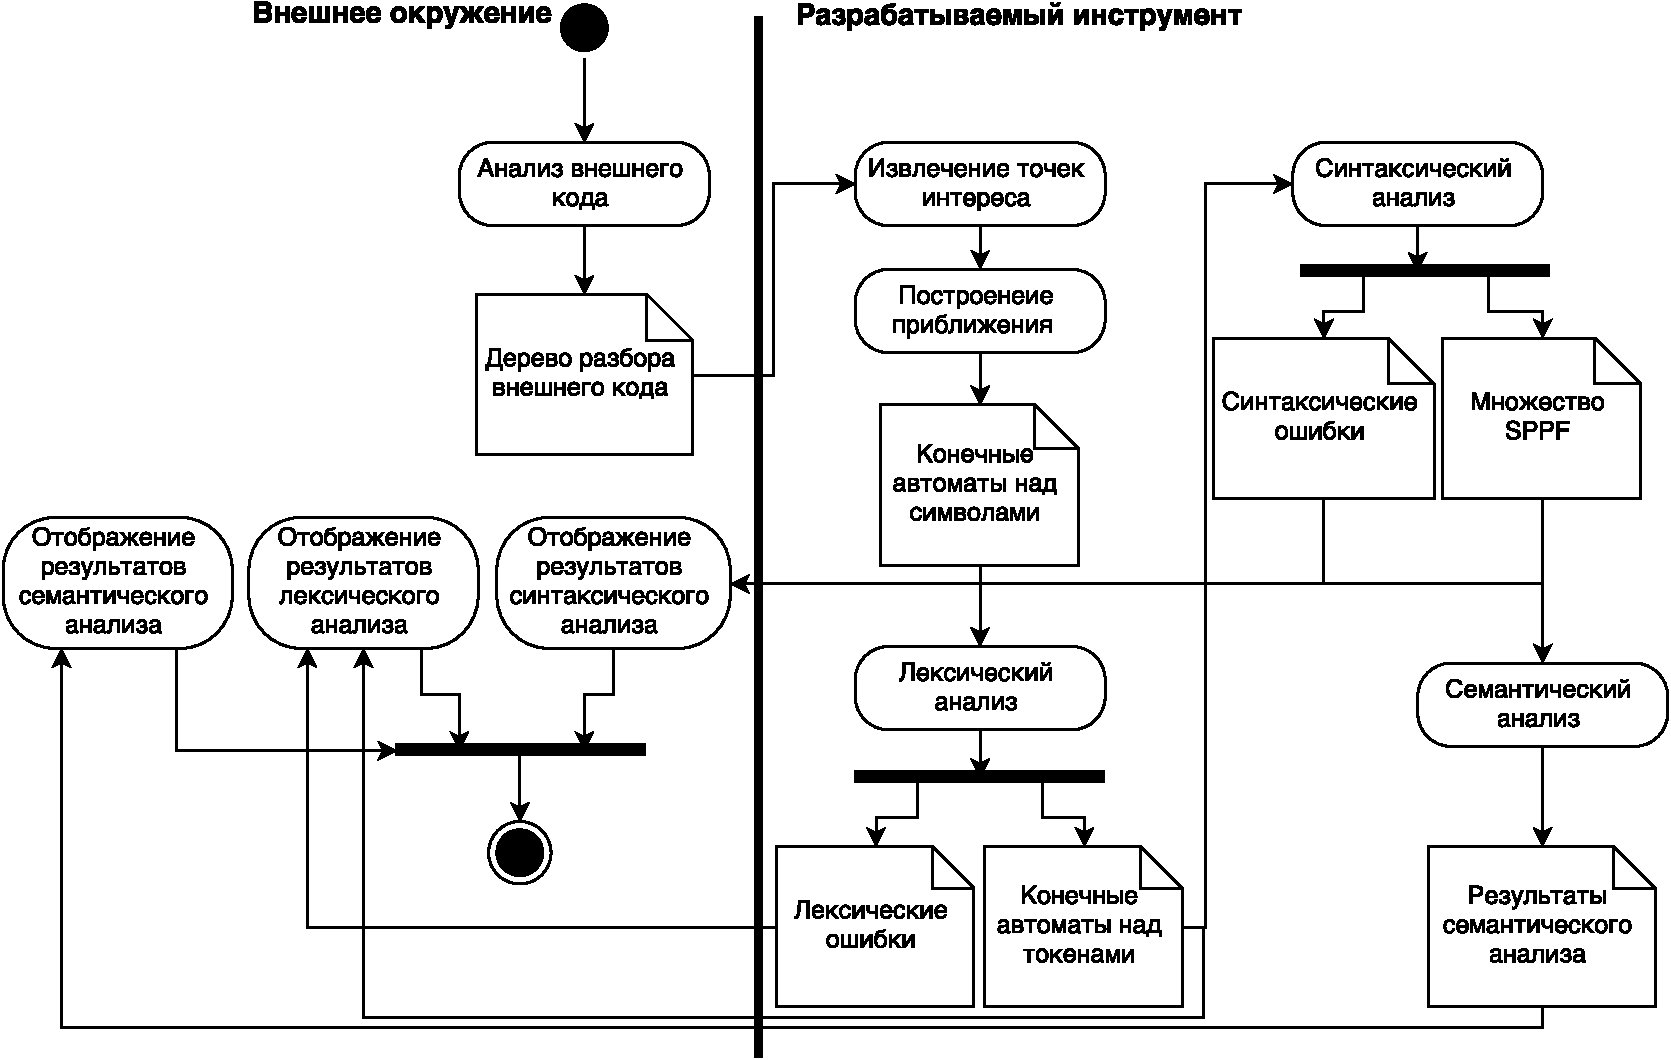
\includegraphics[width=0.95\textwidth]{Activ_SEL_Processing}
 \caption{Пороцесс обработки динамически формируемых выражений}
 \label{sel_processing}
\end{figure}


В \underline{\textbf{четвёртой главе}} описывается метод реинжиниринга встроенного программного кода, основные шаги которого представлены на рисунке~\ref{fig:method}. Данный метод позволяет сформулировать требования к конкретным инструментам обработки встроенного программного кода, необходимым для обработки конкретной информационной системы.

\begin{figure}[]
\begin{center}
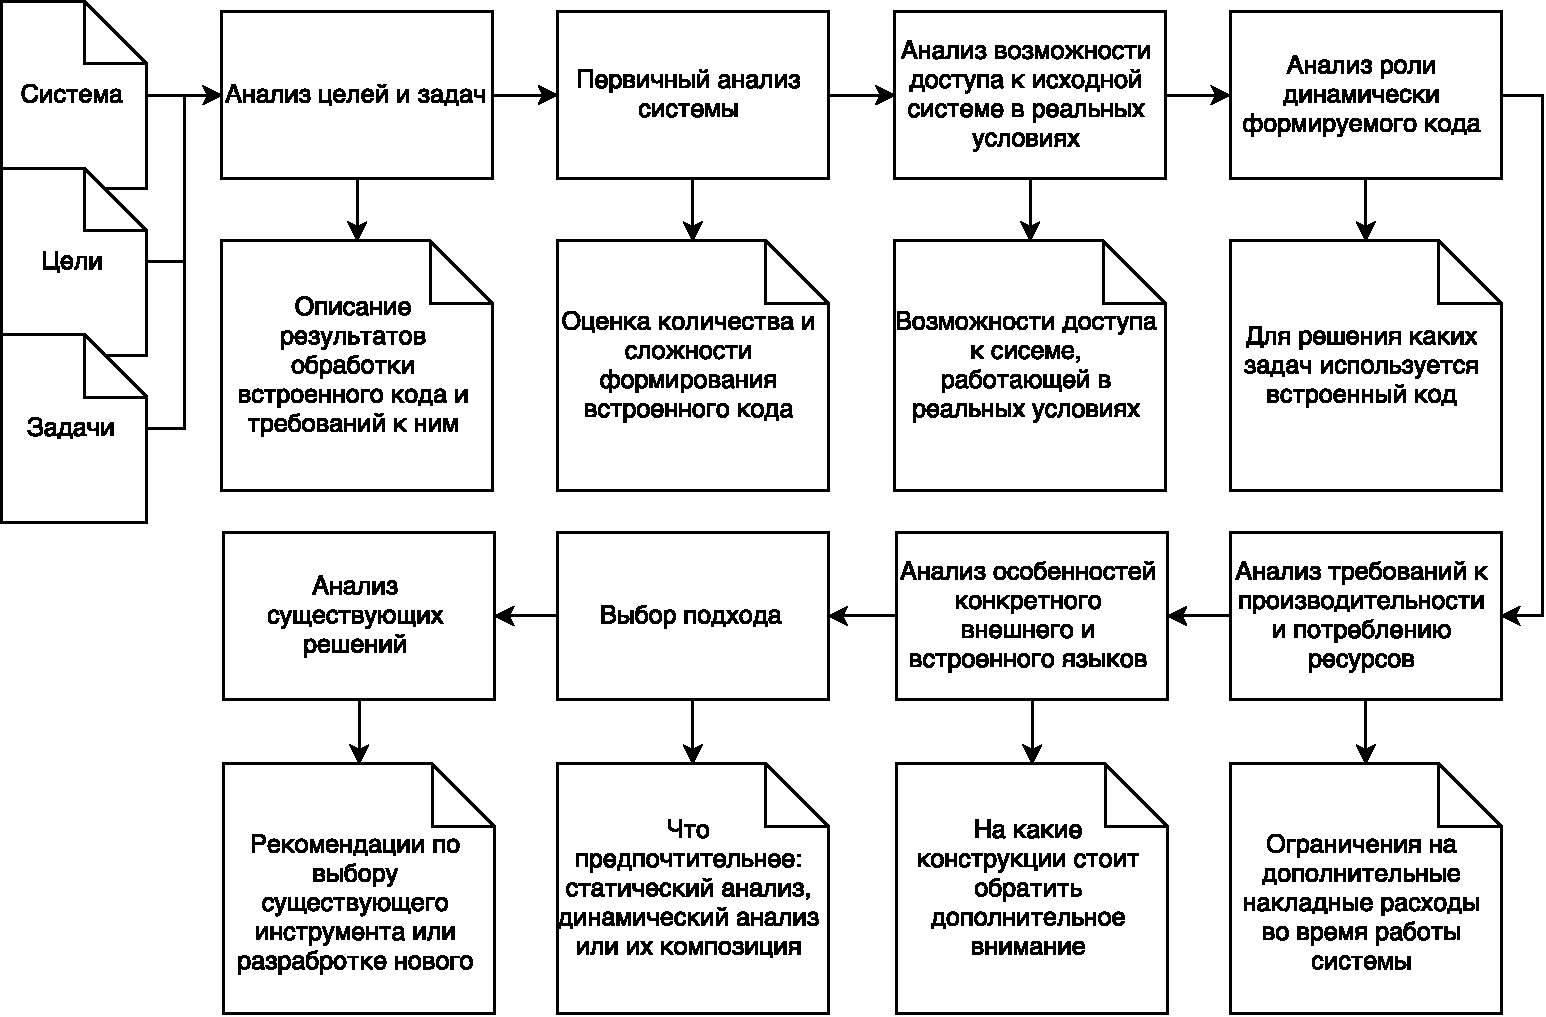
\includegraphics[angle=90,origin=c,width=.95\textwidth]{ReengMethodSteps}
\caption{Основные шаги метода обработки встроенных языков и их результаты}
\label{fig:method} 
\end{center}
\end{figure}


В \underline{\textbf{пятой главе}} приводятся результаты экспериментального исследования YC.SEL.SDK.

Реализованный инструментарий был апробирован в рамках промышленного проекта по миграции базы данных с MS-SQL Server 2005 на Oraclе 11gR2, что позволило оценить предложенную архитектуру и протестировать отдельные компоненты инструментария на реальных данных.

Обрабатываемая система состояла из 850 хранимых процедур и содержала около 2,6 миллионов строк кода. В ней присутствовало 2430 точек выполнения динамических запросов, 75\% этих запросов могли принимать 
более одного значения, при их формировании использовалось от 7 до 212 операторов, среднее количество операторов для формирования запроса равнялось 40.

Алгоритм успешно завершил работу на 2188 входных графах из 2430, аппроксимирующих множества значений запросов. Ручная проверка входных графов, на которых алгоритм завершался с ошибкой, показала, что они действительно не содержали ни одного выражения, корректного в эталонном языке. Причиной этого была либо некорректная работа лексического анализатора, либо наличие в выражениях конструкций, не поддержанных в существующей грамматике. Так как лексический анализатор и грамматика были полностью заимствованы из оригинального проекта, то наличие этих ошибок не является недостатком алгоритма синтаксического анализа. В дальнейшем часть найденых ошибок была исправлена.

Общее время синтаксического анализа составило 27 минут, из них 13 минут было затрачено на разбор графов, не содержащих ни одного корректного выражения, и 4 минуты --- на обработку графа, прерванную по таймауту. На анализ двух графов было затрачено более 2 минут. Распределение входных графов по интервалам времени, затраченным на анализ, приведено на рисунке~\ref{distr}.

\begin{figure}[]
  \centering
 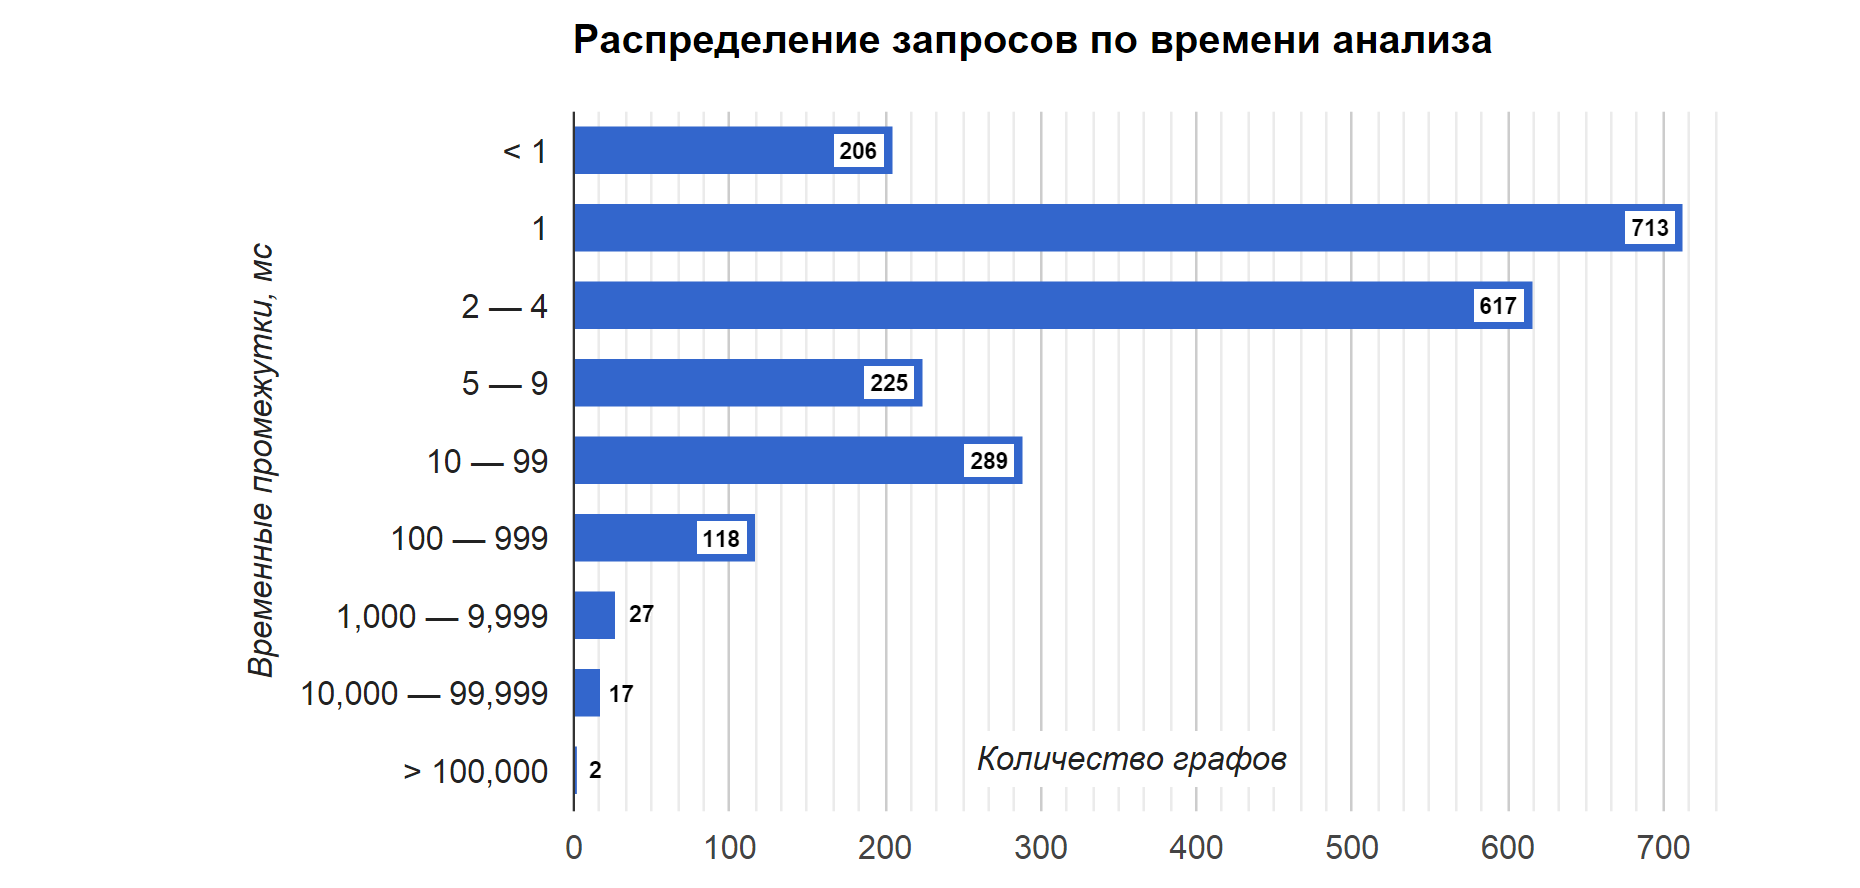
\includegraphics[width=0.95\textwidth]{distr.png}
 \caption{Распределение запросов по времени анализа}
 \label{distr}
\end{figure}


Также было проведено сравнение производительности компоненты синтаксического анализа YC.SEL.SDK с инструментом Alvor. Данный инструмент реализует подход, близкий к представленному в работе, и содержит независимые шаги анализа, что позволяет легко выделить синтаксический анализ, который основан на GLR-алгоритме. Существенным отличием является то, что Alvor не строит деревьев вывода. Важным для успешного проведения измерений является то, что исходный код Alvor опубликован, и это позволило модифицировать его таким образом, чтобы измерить параметры выполнения конкретных методов. 

Так как Alvor не предоставляет средств для простой реализации поддержки новых языков, то для сравнения было выбрано подмножество языка SQL, общее для Alvor и реализованного в рамках апробации инструмента. 
Измерения проводились на синтетических данных, построенных с помощью последовательного соединения базовых блоков, каждый из которых содержит ветвления с $h$ параллельными путями. Результаты экспериментов 
представлены на графике~\ref{fig:YCvsAlvor}. При более чем шестнадцатикратном повторении блоков с $h=2$ время работы Alvor превысило 30 минут и измерения были прекращены. Аналогичная ситуация возникает и при 
более чем десятикратном повторении блоков с $h=3$. Таким образом, измерения показывают, что время работы анализатора Alvor растёт экспоненциально относительно количества повторений базового блока при $h>1$. 
Анализатор созданный на основе YC.SEL.SDK в таких случаях имеет лучшую производительность (до 1000 раз). При этом на линейном входе Alvor работает быстрее. Однако существуют возможности для оптимизации текущей реализации, благодаря чему производительность YC.SEL.SDK на линейном входе может быть улучшена.

\begin{figure}[]
 \centering
 \includegraphics[width=0.95\textwidth]{AlvorVsYCbw.eps}
 \caption{Сравнение производительности Alvor и синтаксического анализатора на базе YC.SEL.SDK}
 \label{fig:YCvsAlvor}
\end{figure}

\underline{\textbf{Шестая глава}} содержит итоги сравнения и соотнесения полученных результатов с существующими аналогами. Получены следующие выводы.
\begin{enumerate}
    \item Разработанный алгоритм синтаксического анализа динамически формируемых выражений является единственным алгоритмом, обрабатывающим регулярную аппроксимацию и строящим конечное представление леса разбора.
    \item Созданная архитектура позволяет предоставить платформу для разработки средств анализа динамически формируемого кода.
    \item Метод реинжиниринга встроенного программного кода сформулирован впервые.
\end{enumerate}



В \underline{\textbf{заключении}} подведены \textbf{итоги} диссертационной работы, которые заключаются в достижении следующих результатов.

\begin{enumerate}
    \item Разработан алгоритм синтаксического анализа динамически формируемых выражений, позволяющий обрабатывать произвольную регулярную аппроксимацию множества значений выражения в точке выполнения, реализующий эффективное управление стеком и гарантирующий конечность представления леса вывода. Доказана завершаемость и корректность предложенного алгоритма при анализе регулярной аппроксимации, представимой в виде произвольного конечного автомата без $\varepsilon$-переходов.
    \item Создана архитектура инструментария для разработки программных средств статического анализа динамически формируемых строковых выражений. На её основе реализован инструментальный пакет для разработки средств статического анализа динамически формируемых выражений, применённый для реализации расширения для ReSharper.
    \item Разработан метод реинжиниринга встроенного программного кода в проектах по реинжинирингу информационных систем. Данный метод применён в проекте компании ЗАО ``Ланит-Терком'' по переносу информационной системы с MS-SQL Server на Oracle Server, для чего реализованы соответствующие программные компоненты.
\end{enumerate}

Кроме этого были сформулированы следующие \textbf{рекомендации по применению результатов работы} в индустрии и научных исследованиях.

\begin{enumerate}
    \item Необходимо, чтобы множество, являющееся аппроксимацией значений динамически формируемого выражения, подаваемое на вход алгоритму синтаксического анализа, было регулярным.
    \item Эталонный язык должен быть описан детерминированной контекстно-свободной грамматикой.
    \item Важно учитывать, что платформа разрабатывалась с ориентацией на создание инструментов для реинжинирига. Поэтому в некоторых компонентах  точность анализа является более приоритетной, чем производительность. Однако архитектура платформы позволяет легко заменять отдельные компоненты и достигать желаемого соотношения точности и производительности инструментов. 
\end{enumerate}

Также были определены \textbf{перспективы дальнейшей разработки тематики}, основными из которых являются исследование возможности выполнения семантических действий непосредственно над SPPF и теоретическая оценка сложности предложенного алгоритма. Кроме этого, с целью обобщения предложенного подхода, а также для получения лучшей производительности и возможностей для более качественной диагностики ошибок необходимо рассмотреть применение других алгоритмов обобщённого синтаксического анализа (GLL, BRNGLR, RIGLR) для решения рассматриваемой задачи.


\newcounter{firstbib}


\renewcommand{\refname}{Публикации автора по теме диссертации в журналах из перечня российских рецензируемых научных журналов, в которых должны быть опубликованы основные научные результаты диссертаций на соискание ученых степеней доктора и кандидата наук}
\begin{thebibliography}{99}
\bibitem{1} Григорьев, С. В. Разработка синтаксических анализаторов в проектах по автоматизированному реинжинирингу информационных систем / Я. А. Кириленко, С. В. Григорьев, Д. А. Авдюхин // Научно-технические ведомости Санкт-Петербургского государственного политехнического университета информатика, телекоммуникации, управление. ---~2013. ---~Т.~3, \textnumero~174. ---~C.~94--98.
\bibitem{2} Григорьев, С. В. Инструментальная поддержка встроенных языков в интегрированных средах разработки / С.~В.~Григорьев, Е.~А.~Вербицкая, М.~И.~Полубелова и др. // Моделирование и анализ информационных систем. ---~2014. ---~Т.~21, \textnumero~6.  ---~С.~131--143.
\bibitem{3} Григорьев, С. В. Обобщенный табличный LL-анализ / С.~В.~Григорьев, А.~К.~Рагозина // Системы и средства информатики. ---~2015. ---~Т.~25, \textnumero~1. ---~С.~89--107. 
\setcounter{firstbib}{\value{enumiv}}
\end{thebibliography}

\renewcommand{\refname}{Публикации автора по теме диссертации в других изданиях}
\begin{thebibliography}{99}
\setcounter{enumiv}{\value{firstbib}}
\bibitem{4} Grigorev, S. GLR-based abstract parsing / S.~Grigorev, I.~Kirilenko // In Proceedings of the 9th Central \& Eastern European Software Engineering Conference in Russia (CEE-SECR ’13). ---~2013. ---~P.~1--9.
\bibitem{5} Grigorev, S. String-embedded language support in integrated development environment / S. Grigorev, E. Verbitskaia, A. Ivanov et al. // Proceedings of the 10th Central and Eastern European Software Engineering Conference in Russia (CEE-SECR '14). ---~2014. ---~P.~1--11.
\bibitem{6} Grigorev, S. From Abstract Parsing to Abstract Translation / S. Grigorev, I. Kirilenko // Proceedings of the Spring/Summer Young Researchers' Colloquium on Software Engineering. ---~2014. ---~P.~1--5.
\bibitem{7} Grigorev, S. Relaxed Parsing of Regular Approximations of String-Embedded Languages / E. Verbitskaia, S. Grigorev, D. Avdyukhin // Preliminary Proceedings of the PSI 2015: 10th International Andrei Ershov Memorial Conference. ---~2015. ---~P.~1--12.

\end{thebibliography}

%\vfill
%\small
%\centering
%\hrule
%\vspace{2.5pt}
%Печать\\
%Печать\\
%Печать\\
%\vspace{2.5pt}
%\hrule
%\vspace{2.5pt}
%Печать\\
%Печать\\
%Печать\\
       % Настройки заглавной странице
\section{Conclusion and future work}
In this paper, we shown how the context-free path query evaluation w.r.t. the relational and the single-path query semantics can be reduced to the calculation of matrix transitive closure. Also, we provided a formal proof of the correctness of the proposed reduction. In addition, we introduced an algorithm for computing this transitive closure, which allows us to efficiently apply GPGPU computing techniques. Finally, we shown the practical applicability of the proposed algorithm by running different implementations of our algorithm on real-world data.

We can identify several open problems for further research. In this paper we have considered only two semantics of context-free path querying but there are other important semantics, such as all-path query semantics~\cite{hellingsPathQuerying} which requires to present all paths for all triples $(A,m,n)$. Context-free path querying implemented with algorithm~\cite{GLL} can answer the queries in all-path query semantics by constructing a parse forest. It is possible to construct a parse forest for a linear input by matrix multiplication~\cite{okhotin_cyk}. Whether it is possible to generalize this approach for a graph input is an open question.

In our algorithm, we calculate the matrix transitive closure naively, but there are algorithms for the transitive closure calculation, which are asymptotically more efficient. Therefore, the question is whether it is possible to apply these algorithms for the matrix transitive closure calculation to the problem of context-free path querying.

Also, there are Boolean grammars~\cite{okhotinBoolean}, which have more expressive power than context-free grammars. Boolean path querying is an undecidable problem~\cite{hellingsRelational} but our algorithm can be trivially generalized to work on boolean grammars because parsing with boolean grammars can be expressed by matrix multiplication~\cite{okhotin_cyk}. It is not clear what a result of our algorithm applied to Boolean grammars would look like. Our hypothesis is that it would produce the upper approximation of a solution.

From a practical point of view, matrix multiplication in the main loop of the proposed algorithm may be performed on different GPGPU independently. It can help to utilize the power of multi-GPU systems and increase the performance of context-free path querying.

There is an algorithm~\cite{apspGPU} for transitive closure calculation on directed graphs which generalized to handle graph sizes inherently larger then the DRAM memory available on the GPU. Therefore, the question is whether it is possible to apply this approach to the matrix transitive closure calculation in the problem of context-free path querying.    % Последние слайды презентации
\appendix
\section{Dataset description}\label{section:dataset}

In our evaluation we use dataset which contains the following parts.
{\setlength{\tabcolsep}{0.4em}
	\begin{table}[h]
		\caption{RDFs properties}
		\label{tbl:propRDF}
		\rowcolors{2}{}{lightgray}
		\begin{tabular}{| l | c | c | c | c |}
			\hline
			Name                  & \#V    & \#E     & \#type &\#subClassOf \\
			\hline
			\hline
			atom-primitive				& 291		& 685		& 138	& 122	\\
			univ-bench					& 179		& 413		& 84		& 36		\\
			travel						& 131		& 397		& 90		& 30		\\
			skos							& 144		& 323		& 70		& 1		\\
			people\_pets					& 337		& 834		& 161	& 33		\\
			generations					& 129		& 351		& 78		& 0		\\
			foaf							& 256		& 815		& 174	& 10		\\
			biomed-mesure-prim   	    & 341		& 711		& 130	& 122	\\
			funding						& 778		& 1480		& 304	& 90               \\
			pizza						& 671		& 2604		& 365	& 259              \\
			wine							& 733		& 2450		& 485	& 126              \\
			core							& 1323		& 8684		& 1412	& 178              \\
			pathways						& 6238		& 37196		& 3118 	& 3117             \\
			go-hierarchy					& 45007		& 1960436	& 0		& 490109           \\
			enzyme						& 48815		& 219390		& 14989	& 8163             \\
			eclass\_514en				& 239111		& 1047454	& 72517	& 90962            \\
			go							& 272770		& 1068622	& 58483	& 90512            \\
			\hline
		\end{tabular}
	\end{table}
}

{\setlength{\tabcolsep}{0.4em}
\begin{table*}[h]
\caption{RDFs query $G_2$ (time is measured in seconds and memory is measured in megabytes)}
\label{tbl:tableRDFQ2}
\rowcolors{3}{}{lightgray}
\begin{tabular}{| l | r  r | r  r | r  r | r  r | r  r |}
    \hline

    \multirow{3}{*}{Name}   &   \multicolumn{6}{|c|}{Relational semantics index}	&	\multicolumn{4}{|c|}{Single path semantics index} \\
    \cline{2-11}
    &	\multicolumn{2}{|c|}{RG\_CPU\textsubscript{rel}}	&	\multicolumn{2}{|c|}{RG\_CUSP\textsubscript{rel}}	&	\multicolumn{2}{|c|}{RG\_SPARSE\textsubscript{rel}} &	\multicolumn{2}{|c|}{RG\_CPU\textsubscript{path}}	&	\multicolumn{2}{|c|}{RG\_SPARSE\textsubscript{path}}	 \\
    \cline{2-11}
    &   Time & Mem &  Time     & Mem & Time     & Mem  &  Time     & Mem & Time     & Mem \\
    \hline
    \hline
    atom-primitive          & 0.001 & 0.3  & 0.001 & 0.1 & 0.002 & 0.1   & 0.001 & 0.3  & 0.002 & 0.1   \\
biomedical-mesure-primitive & 0.002 & 0.1  & 0.014 & 2.0   & 0.009 & 0.1   & 0.006 & 0.1  & 0.012 & 0.1   \\
core                        & 0.001 & 0.3  & 0.006 & 0.1 & 0.004 & 0.1   & 0.003 & 0.3  & 0.005 & 0.1   \\
eclass\_514en               & 0.035 & 6.5  & 0.020 & 16.0  & 0.100   & 12.0    & 0.123 & 17.7 & 0.127 & 18.0    \\
enzyme                      & 0.006 & 3.9  & 0.006 & 0.6 & 0.010  & 0.1   & 0.012 & 5.3  & 0.008 & 0.4   \\
foaf                        & 0.001 & 0.1  & 0.004 & 0.1 & 0.002 & 0.1   & 0.001 & 0.1  & 0.003 & 0.1   \\
funding                     & 0.002 & 0.1  & 0.015 & 0.4 & 0.007 & 0.1   & 0.009 & 0.1  & 0.008 & 0.1   \\
generations                 & 0.001 & 0.1  & 0.001 & 0.1 & 0.001 & 0.1   & 0.001 & 0.1  & 0.001 & 0.1   \\
go-hierarchy                & 0.095 & 17.8 & 0.253 & 528.0 & 0.175 & 130.4 & 0.884 & 88.8 & 0.306 & 138.8 \\
go                          & 0.306 & 25.8 & 0.240 & 84.0  & 0.181 & 25.4  & 0.918 & 78.1 & 0.219 & 34.2  \\
pathways                    & 0.005 & 0.2  & 0.005 & 0.4 & 0.004 & 0.1   & 0.017 & 0.5  & 0.003 & 0.1   \\
people\_pets                & 0.001 & 0.1  & 0.007 & 0.1 & 0.004 & 0.1   & 0.001 & 0.1  & 0.005 & 0.1   \\
pizza                       & 0.002 & 0.3  & 0.012 & 0.2 & 0.008 & 0.1   & 0.010  & 0.3  & 0.009 & 0.1   \\
skos                        & 0.001 & 0.1  & 0.001 & 0.1 & 0.001 & 0.1   & 0.001 & 0.1  & 0.002 & 0.1   \\
travel                      & 0.001 & 0.1  & 0.007 & 0.1 & 0.005 & 0.1   & 0.001 & 0.1  & 0.005 & 0.1   \\
univ-bench                  & 0.001 & 0.1  & 0.007 & 0.1 & 0.005 & 0.1   & 0.001 & 0.1  & 0.005 & 0.1   \\
wine                        & 0.001 & 0.3  & 0.006 & 0.1 & 0.004 & 0.1   & 0.002 & 0.3  & 0.004 & 0.1  \\
    \hline
  \end{tabular}
\end{table*}
}

\begin{itemize}
\item The real-world data RDFs provided in CFPQ\_Data dataset\footnote{CFPQ\_Data dataset GitHub repository: \url{https://github.com/JetBrains-Research/CFPQ_Data}. Access date: 12.11.2019.} from~\cite{Mishin:2019:ECP:3327964.3328503}.
\item Geospecies (RDF which contains information about biological hierrarchy\footnote{The Geospecies RDF: \url{https://old.datahub.io/dataset/geospecies}. Access date: 12.11.2019.} and same-generation query over \textit{broaderTransitive} relation) is provided in~\cite{Kuijpers:2019:ESC:3335783.3335791} and integrated in our evaluation with CFPQ\_Data.
\item It was shown in~\cite{Mishin:2019:ECP:3327964.3328503} that matrix-based algorithm is performant enough to handle bigger RDFs than those used in the initial datasets, such as~\cite{RDF}.
So, we add several big RDFs to CFPQ\_Data and use them in our evaluation.
New RDFs: \textit{go-hierarchy, go, enzime, core, pathways} are from UniProt database\footnote{Protein sequences data base: \url{https://www.uniprot.org/}. RDFs with data are avalable here: \url{ftp://ftp.uniprot.org/pub/databases/uniprot/current_release/rdf}. Access date: 12.11.2019}, and \textit{eclass-514en} is from eClassOWL project\footnote{eClassOWL project: \url{http://www.heppnetz.de/projects/eclassowl/}. eclass-514en file is available here: \url{http://www.ebusiness-unibw.org/ontologies/eclass/5.1.4/eclass_514en.owl}. Access date: 12.11.2019.}.
\end{itemize}

The properties of the RDFs from the dataset are given in table \ref{tbl:propRDF}. 
Geospecies RDF contains 450609 vertices, 2311461 edges, and 20867 edges labeled by \textit{broaderTransitive}.
Note that while the number of edges labeled by \textit{broaderTransitive} is equal to provided in~\cite{Kuijpers:2019:ESC:3335783.3335791}, the total number of vertices and edges is bigger. It is because we naively convert each triple from RDF to edge in the graph, while J. Kuijpers et al. use special \textit{neosemantics}\footnote{Neosemantix is an RDF processing plugin for Neo4j. Web page: \url{https://neo4j.com/labs/nsmtx-rdf/}. Access date: 30.03.2020.} plugin which can, for example, handling multivalued properties accurately.  

The variants of the \textit{same-generation query}~\cite{FndDB} are used in almost all cases because it is an important example of real-world queries that are context-free but not regular.
So, variations of the same generation query are used in our evaluation.
All queries are added to the CFPQ\_Data dataset.

We use two queries over \textit{subClassOf} and \textit{type} relations.
The first query is the grammar $G_1$:
\[
 \begin{array}{lcl}
   s  \rightarrow \textit{subClassOf}^{\ -1} \ s \ \textit{subClassOf}   & \quad & s  \rightarrow \textit{type}^{\ -1} \ s \ \textit{type}     \\
   s  \rightarrow \textit{subClassOf}^{\ -1} \ \textit{subClassOf}       & \quad & s  \rightarrow  \textit{type}^{\ -1}  \ \textit{type}

 \end{array}
 \]
The second one is the grammar $G_2$: \[s \rightarrow \textit{subClassOf}^{\ -1} \ s \ \textit{subClassOf} \mid \textit{subClassOf}\]

For geospecies we use same-generation query \textit{geo} from the original paper~\cite{Kuijpers:2019:ESC:3335783.3335791}: \[s \rightarrow \textit{broaderTransitive} \ s \ \textit{broaderTransitive}^{\ -1} \]
\[s \rightarrow \textit{broaderTransitive}  \ \textit{broaderTransitive}^{\ -1} \]


\section{Evaluation Details}

Results for RDFs querying with $G_2$ grammar are presented in table~\ref{tbl:tableRDFQ2}.
We can see, that for small graphs time for both relational and single-path querying are similar for CPU and GPGPU versions, but for bigger graphs (\textit{go} and \textit{go-hierarchy}, for example) GPUPU version is more performant than CPU one.

\balance

      % Запасные слайды презентации
\end{document}
